% This file was converted to LaTeX by Writer2LaTeX ver. 1.0.2
% see http://writer2latex.sourceforge.net for more info
\documentclass[a4paper,openany,10pt]{memoir}
\usepackage[utf8]{inputenc}
\usepackage[T1]{fontenc}
\usepackage[english,spanish]{babel}
\usepackage{amsmath}
\usepackage{amssymb,amsfonts,textcomp}
\usepackage{color}
\usepackage{array}
\usepackage{hhline}
\usepackage{hyperref}
\hypersetup{pdftex, colorlinks=true, linkcolor=blue, citecolor=blue, filecolor=blue, urlcolor=blue, pdftitle=, pdfauthor=, pdfsubject=, pdfkeywords=}
\usepackage[pdftex]{graphicx}
\usepackage{xspace}
\usepackage{todonotes}
\usepackage{savetrees}
\usepackage{tikz}


% Text styles
\newcommand\textstylenombreprograma[1]{\texttt{\textbf{\textsl{#1}}}}
\newcommand\textstyleGUIELEMENT[1]{\textrm{\textbf{\textit{#1}}}}
\newcommand\textstyleUserEntry[1]{\texttt{#1}}
\newcommand\textstylekonsolecomment[1]{\texttt{\textit{#1}}}
\newcommand\textstyleGUIELEMENTREDUCED[1]{\textrm{\textbf{\textit{#1}}}}
\newcommand\textstyleMainindexentry[1]{\textbf{#1}}
\newcommand\textstylePageNumber[1]{#1}
% Outline numbering
\setcounter{secnumdepth}{3}
\renewcommand\thesection{\arabic{section}}
\renewcommand\thesubsection{\arabic{section}.\arabic{subsection}}
\renewcommand\thesubsubsection{\arabic{section}.\arabic{subsection}.\arabic{subsubsection}}
% List styles
\newcounter{saveenum}
\newcommand\liststyleLi{%
\renewcommand\labelitemi{{}--}
\renewcommand\labelitemii{{}--}
\renewcommand\labelitemiii{{}--}
\renewcommand\labelitemiv{{}--}
}
\newcommand\liststyleLii{%
\renewcommand\labelitemi{{}--}
\renewcommand\labelitemii{{}--}
\renewcommand\labelitemiii{{}--}
\renewcommand\labelitemiv{{}--}
}
\newcommand\liststyleLiii{%
\renewcommand\labelitemi{{\textbullet}}
\renewcommand\labelitemii{{\textbullet}}
\renewcommand\labelitemiii{{\textbullet}}
\renewcommand\labelitemiv{{\textbullet}}
}
\newcommand\liststyleLiv{%
\renewcommand\theenumi{\alph{enumi}}
\renewcommand\theenumii{\arabic{enumii}}
\renewcommand\theenumiii{\arabic{enumiii}}
\renewcommand\theenumiv{\arabic{enumiv}}
\renewcommand\labelenumi{\theenumi)}
\renewcommand\labelenumii{\theenumii.}
\renewcommand\labelenumiii{\theenumiii.}
\renewcommand\labelenumiv{\theenumiv.}
}
\newcommand\liststyleLv{%
\renewcommand\theenumi{\alph{enumi}}
\renewcommand\theenumii{\alph{enumii}}
\renewcommand\theenumiii{\arabic{enumiii}}
\renewcommand\theenumiv{\arabic{enumiv}}
\renewcommand\labelenumi{\theenumi)}
\renewcommand\labelenumii{\theenumii)}
\renewcommand\labelenumiii{\theenumiii.}
\renewcommand\labelenumiv{\theenumiv.}
}
\newcommand\liststyleLvi{%
\renewcommand\theenumi{\arabic{enumi}}
\renewcommand\theenumii{\arabic{enumii}}
\renewcommand\theenumiii{\arabic{enumiii}}
\renewcommand\theenumiv{\arabic{enumiv}}
\renewcommand\labelenumi{\theenumi)}
\renewcommand\labelenumii{\theenumii.}
\renewcommand\labelenumiii{\theenumiii.}
\renewcommand\labelenumiv{\theenumiv.}
}
\newcommand\liststyleLvii{%
\renewcommand\labelitemi{{}--}
\renewcommand\labelitemii{{}--}
\renewcommand\labelitemiii{{}--}
\renewcommand\labelitemiv{{}--}
}
\newcommand\liststyleLviii{%
\renewcommand\theenumi{\arabic{enumi}}
\renewcommand\theenumii{\arabic{enumii}}
\renewcommand\theenumiii{\arabic{enumiii}}
\renewcommand\theenumiv{\arabic{enumiv}}
\renewcommand\labelenumi{\theenumi)}
\renewcommand\labelenumii{\theenumii.}
\renewcommand\labelenumiii{\theenumiii.}
\renewcommand\labelenumiv{\theenumiv.}
}
\newcommand\liststyleLix{%
\renewcommand\labelitemi{{}--}
\renewcommand\labelitemii{{}--}
\renewcommand\labelitemiii{{}--}
\renewcommand\labelitemiv{{}--}
}
\newcommand\liststyleLx{%
\renewcommand\theenumi{\arabic{enumi}}
\renewcommand\theenumii{\arabic{enumii}}
\renewcommand\theenumiii{\arabic{enumiii}}
\renewcommand\theenumiv{\arabic{enumiv}}
\renewcommand\labelenumi{\theenumi)}
\renewcommand\labelenumii{\theenumii.}
\renewcommand\labelenumiii{\theenumiii.}
\renewcommand\labelenumiv{\theenumiv.}
}
% Page layout (geometry)
% \setlength\voffset{-1in}
% \setlength\hoffset{-1in}
% \setlength\topmargin{2cm}
% \setlength\oddsidemargin{5cm}
% \setlength\textheight{24.776667cm}
% \setlength\textwidth{16.999cm}
\setlength\footskip{26.144882pt}
% \setlength\headheight{3cm}
\setlength\headsep{0.5cm}

\setlrmarginsandblock{2.5cm}{5cm}{*}
\setulmarginsandblock{2.5cm}{2.5cm}{*}
\checkandfixthelayout

% Footnote rule
\setlength{\skip\footins}{0.119cm}
\renewcommand\footnoterule{\vspace*{-0.018cm}\setlength\leftskip{0pt}\setlength\rightskip{0pt plus 1fil}\noindent\textcolor{black}{\rule{0.25\columnwidth}{0.018cm}}\vspace*{0.101cm}}
% Pages styles
\makeatletter
\newcommand\ps@Standard{
  \renewcommand\@oddfoot{}
  \renewcommand\@oddhead{\hspace{-3cm}\textstylePageNumber{\ }\textstylePageNumber{v\appversion, 16-oct-2013\hfill Manual de la usuaria de \appname\hfill Página }\thepage{}}
  \renewcommand\@evenhead{\@oddhead}
  \renewcommand\@evenfoot{\@oddfoot}
  \renewcommand\thepage{\arabic{page}}
}
\newcommand\ps@FirstPage{
  \renewcommand\@oddhead{}
  \renewcommand\@evenhead{}
  \renewcommand\@oddfoot{}
  \renewcommand\@evenfoot{}
  \renewcommand\thepage{\arabic{page}}
}
\newcommand\ps@Primeraprimerapagina{
  \renewcommand\@oddhead{}
  \renewcommand\@evenhead{}
  \renewcommand\@oddfoot{}
  \renewcommand\@evenfoot{}
  \renewcommand\thepage{\arabic{page}}
}
\makeatother
\pagestyle{Standard}
% Non-floating captions
\makeatletter
\newcommand\captionof[1]{\def\@captype{#1}\caption}
\makeatother
\title{}
\author{}
\date{2008-12-08}

\newcommand{\menu}[1]{\textbf{#1}}
\newcommand{\directorio}[1]{\textbf{#1}}
\newcommand{\filename}[1]{\texttt{#1}}
\newcommand{\commercialname}[1]{\textsc{#1}}
\newcommand{\hint}[1]{\textit{#1}\par}
\newcommand{\recuadro}[2]{#1\par#2\par}
\newcommand{\notamargen}[1]{\marginpar{\color{green}\backgroundcolor{blue}#1}}
\newcommand{\truco}[1]{\colorbox{gray!20!white}{\begin{minipage}{\textwidth}#1\end{minipage}}}

\let\oldmarginpar\marginpar
% renew the \marginpar command to draw 
% a node; it has a default setting which 
% can be overwritten
\renewcommand{\marginpar}[2][rectangle,draw,fill=orange,rounded corners, text width= 4cm]{%
        \oldmarginpar{%
        \tikz \node at (0,0) [#1]{#2};}%
        }

\begin{document}

\tableofcontents

%\newcommand{\appname}{LosPajaros\xspace}
\newcommand{\appversion}{0.1.0}
\newcommand{\appdescription}{gestión de cantina y tienda\xspace}
\newcommand{\appreleasedate}{8 de diciembre de 2012}
\newcommand{\organizacion}{asociación\xspace}
\newcommand{\Organizacion}{Asociación\xspace}
\newcommand{\organizaciones}{asociaciones\xspace}

\newcommand{\appname}{GestiONG\xspace}
\newcommand{\appversion}{0.4.0}
\newcommand{\appdescription}{gestión comercial y contable para asociaciones sin ánimo de lucro\xspace}
\newcommand{\appreleasedate}{8 de diciembre de 2012}
\newcommand{\organizacion}{asociación\xspace}
\newcommand{\organizaciones}{asociaciones\xspace}
\newcommand{\Organizacion}{Asociación\xspace}
% \newcommand{\appname}{GestiONG\xspace}
\newcommand{\appversion}{0.4.0}
\newcommand{\appdescription}{gestión comercial y contable para empresas\xspace}
\newcommand{\appreleasedate}{8 de diciembre de 2012}
\newcommand{\organizacion}{empresa\xspace}
\newcommand{\Organizacion}{empresa\xspace}
\newcommand{\organizaciones}{empresas\xspace}

% \input{ecotiendag_commands.tex}


\chapter{Bienvenida}
\section{¿Qué es \appname?}

\appname es parte de ProgramacionSocial.net.


GestiONG es una filosofía.


\appname es un programa para la \appdescription desarrollado bajo el paradigma del
software libre con el objetivo de ser utilizado en sistemas operativos
libres como GNU/Linux. La versión actual permite la gestión de la
base social: contactos, altas y bajas, cuotas, \ldots; la gestión
contable adaptada al nuevo plan del 2008 y una completa gestión
económica de proyectos, incluyendo remesas de recibos y gastos e
ingresos por partidas.

\section{¿Cuál es el modelo de negocio de \appname?}

\appname es libre y la base general del software es además gratuita. 
El modelo de negocio consiste en dos vías:
\begin{itemize}
 \item Cobrar por el trabajo efectivo de instalación, puesta en marcha y formación al cliente.
 \item Cobrar por el desarrollo de módulos específicos para cada cliente.
\end{itemize}


\section{¿A quién va dirigido \appname?}
\appname permite llevar la contabilidad de una organización sin
ánimo de lucro a personas no expertas en informática ni en
contabilidad: tesoreras, secretarias e incluso voluntarias. Se ha
realizado un gran esfuerzo, por un lado, para que el manejo del
programa sea fácil, intuitivo y seguro sin necesidad de saber
informática y por otro lado, para llevar la contabilidad oficial sin
necesidad de saber contabilidad.

\appname es, además, un proyecto posicionado firmemente en cuestiones
que atañen a la libertad de uso, al tipo de organizaciones a las que
va destinado y al uso del lenguaje de los manuales y de los textos del
programa.

En cuanto a la libertad, todo el proyecto, incluyendo diseño,
código, documentación e imágenes está distribuido bajo una
serie de licencias conocidas genéricamente como copyleft. Estas
licencias promueven la distribución, uso y modificación libre de
cualquier parte del proyecto respetando los derechos de autoría e
intentando evitar su apropiación por parte de terceras personas. El
código está licenciado bajo la Licencia Pública General GNU (GPL,
GNU General Public Licence) y la documentación bajo la Licencia de
Documentación Libre de GNU (GNU Free Public License). El compromiso
de \appname con el software libre llega hasta el punto de no apoyar su
empleo en sistemas operativos propietarios ni formatos de documentos
que no sean libres. Esta decisión de diseño ha retrasado, quizás,
la adopción del proyecto por parte de organizaciones que aún no
estaban preparadas para el cambio efectivo de mentalidad, pero aún
así, \appname se ha mantenido, y espera mantenerse en el futuro, fiel
a sus principios.

En cuanto al tipo de organizaciones a las que va destinado, \appname se
posiciona a favor de las organizaciones sin ánimo de lucro: ONG,
asociaciones y clubes de todo tipo, cooperativas de trabajo, centros
sociales, organismos públicos, etc. En este sentido, las necesidades
de organizaciones con ánimo de lucro serán simplemente desoídas.

Por último, en cuanto al lenguaje empleado, se ha preferido el uso del
femenino genérico no solo en el programa y en la documentación,
sino también en el propio código fuente, lo cual ha sido un
desafío que nos ha mostrado hasta qué punto está arraigado el
lenguaje sexista en las carreras técnicas.

\section{¿Qué se puede hacer con \appname?}
Si bien es cierto que la apariencia de \appname es simple, por dentro
está diseñado para crecer. La mayor parte del esfuerzo de
programación se ha empleado en crear una base que pueda ser extendida
por cada organización; por eso, esta primera versión de
producción ofrece una funcionalidad básica para la gestión
contable, de socias y de proyectos a la espera de conocer las
necesidades reales de las asociaciones. 

\section{Sensibilidades}

\appname es un proyecto dentro de ProgramacionSocial.net. Esto le confiere
una serie de sensibilidades:

\begin{itemize}
 \item Traer la potencia y eficacia de la gestión empresarial a las organizaciones sociales.
 \item Utilizar el femenino genérico.
 \item Apuesta comprometida por el software libre.
 \item Apuesta por lo local.
\end{itemize}


La versión actual permite:

\liststyleLi
\begin{itemize}
\item Puesta en marcha inmediata:

\begin{itemize}
\item Importar los datos de las personas socias desde cualquier hoja de
cálculo.
\item Importar \ cuentas y asientos desde otros programas de
contabilidad.
\end{itemize}
\end{itemize}
\liststyleLii
\begin{itemize}
\item Gestión de las personas socias de la asociación:

\begin{itemize}
\item Dar de alta los datos de contacto y mantener las altas y bajas de
las personas socias.
\item Definir las cuotas y formas de pago de cada persona socia.
\item Producir informes de socias, remesas, recibos, etc.
\item Facilitar el envío masivo de correspondencia y emails.
\end{itemize}
\item Gestión de proyectos:

\begin{itemize}
\item Crear remesas de recibos y enviarlas a las cajas de ahorros y
bancos.
\item Controlar los pagos, impagos y devoluciones de los recibos.
\item Definir las diferentes partidas de gastos e ingresos para cada
proyecto.
\item Asignar cada apunte contable a una partida determinada de un
proyecto.
\item Producir informes de gastos e ingresos por partidas para cada
proyecto.
\item Añadir miembros a los proyectos, con su tipo de filiación y
forma de pago y generar remesas del mismo modo que con las personas
socias.
\end{itemize}
\item Gestión contable:

\begin{itemize}
\item Crear automáticamente el plan contable estándar del 2008 o el
del 1998.
\item Introducir asientos manualmente y a partir de asientos tipo.
\item Producir informes de sumas y saldos, balances, extractos, etc.
\end{itemize}
\item General:

\begin{itemize}
\item Exportar cualquier fichero para: hojas de cálculo, combinación
de correspondencia, envíos masivos de correos electrónicos, etc.
\item Modificar y añadir informes nuevos.
\item Generar informes en PDF, OpenOffice, HTML, etc.
\end{itemize}
\end{itemize}

\bigskip

\section{Características de \appname}

\begin{description}
 \item[Facilidad de instalación y puesta en marcha.]
\appname no presupone ningún conocimiento sobre informática por
parte de la usuaria. Las instrucciones para la instalación y puesta
en marcha son lo suficientemente detalladas y precisas para que el
programa se pueda descargar de Internet e instalar sin problemas. Una
vez instalado, el programa se encarga de crear la base de datos. Una
vez puesto en marcha, hay numerosas opciones para importar los datos de
vuestra organización y comenzar a trabajar inmediatamente.

\item[Facilidad de uso.]
La aplicación permite trabajar con varios ficheros y documentos
simultáneamente. La introducción de datos se ha diseñado para que
sea lo más cómoda y correcta posible, pensando en todo momento en
agilizar el proceso mediante un uso eficientemente el teclado. Todos
los ficheros presentan un aspecto y comportamiento similar con una gran
cantidad de opciones para búsqueda, filtro, ordenación,
impresión, duplicación, importación, exportación, etc.

\item[Simplicidad.]

\appname reduce al máximo la cantidad de datos que la usuaria debe
introducir y maximiza la información que se obtiene de ellos. Así,
cada vez que se introduce un gasto o un ingreso, el programa genera
automáticamente el asiento contable correspondiente. Además, si se
indica la partida a la que pertenece el gasto o ingreso, se mantienen
actualizadas las partidas de gastos e ingresos del proyecto. Cuando se
paga un recibo, además de generarse el asiento contable
correspondiente, se puede imprimir inmediatamente el \textit{recibí}
para la persona socia.


\item[Adaptabilidad.]
\appname puede ser configurado en diversos aspectos para adaptarlo a
cualquier tipo de asociación u organización. 

\liststyleLiii
\begin{itemize}
\item Puede ser usado en cualquier idioma, con cualquier formato de
moneda y fecha.
\item Permite modificar las descripciones de los ficheros y \ campos de
la base de datos para que se ajusten a la nomenclatura de cada
organización.
\item Soporte para múltiples asociaciones, múltiples ejercicios y
múltiples usuarias.
\item Permite la modificación y creación de nuevos informes.
\end{itemize}

\item[Extensibilidad.]
La versión básica posee tres módulos: gestión de socias,
gestión de proyectos y contabilidad. Pero esta base la puede extender
cualquier programadora para desarrollar nuevos módulos o adaptar los
ya existentes. Hasta la fecha, se ha desarrollado un módulo de
gestión de atenciones para una asociación de apoyo a las
trabajadoras del sexo y se está desarrollando un módulo para
inscripciones a talleres y cursos y otro módulo para la gestión de
una biblioteca/mediateca.


\item[Independencia.]
La adhesión al software libre y a los estándares abiertos asegura
que vuestros datos estarán controlados siempre por vuestra
organización y que podréis, llegado el caso, migrarlos a cualquier
otro formato sin ningún tipo de problemas.

\end{description}



\section{Organización de este manual}
El capítulo II comienza con tres tutoriales con instrucciones muy
detalladas y profusamente ilustradas: instalación; puesta en marcha y
comienzo del trabajo efectivo. El objetivo es poner en marcha \appname
en vuestra organización independientemente de los conocimientos
informáticos que poseáis.

Los siguientes capítulos, necesariamente incompletos aún, realizan
un somero análisis de cada módulo del sistema: III Gestión de las
personas socias, IV Gestión de proyectos y \ V Gestión contable.

Los últimos capítulos contienen información sobre otros aspectos
de \appname que permitirán un uso más efectivo del mismo: VI)
Configuración; VII) Generación de informes; VIII) Herramientas del
sistema.




\chapter{Instalación de GestiONG}

\section{Instalación}
Dependiendo de la distribución de GNU/Linux que utilices, la
instalación de GestiONG será diferente. Si tienes un PC con
\textstylenombreprograma{Debian}, \textstylenombreprograma{Ubuntu} (o
alguna de sus variedades como \textstylenombreprograma{Kubuntu},
\textstylenombreprograma{Xubuntu}, ... ),
\textstylenombreprograma{Fedora}, \textstylenombreprograma{Red Hat} o
\textstylenombreprograma{Mandriva}, estás de enhorabuena porque
GestiONG proporciona paquetes preparados para su instalación de forma
sencilla. Para otras distribuciones, otros tipos de ordenador (como los
Mac) u ordenadores muy antiguos, necesitarás construir el programa
tú misma.

\subsection{Usando paquetes preparados para tu sistema}
En la página de descarga del proyecto,
\href{http://sourceforge.net/project/showfiles.php?group_id=80104&package_id=81685&release_id=578703}{https://sourceforge.net/project/showfiles.php?group\_id=80104}
encontrarás una lista de paquetes disponibles para distintas
arquitecturas de computadoras y distribuciones de GNU/Linux. 



\begin{center}
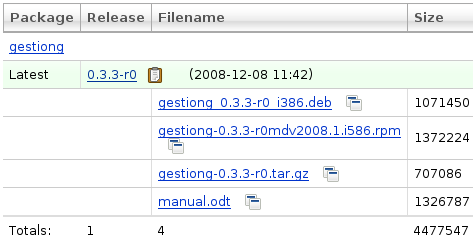
\includegraphics[width=7.915cm,height=4.166cm]{manual-img1.png}
\captionof{figure}[Zona de descarga desde sourceforge.net]{Zona de
descarga desde sourceforge.net}

\end{center}
Haz click sobre el fichero correspondiente a tu distribución: para
\ \textstylenombreprograma{Fedora}, \textstylenombreprograma{Mandriva}
y \textstylenombreprograma{Red Hat}, elige:

\ \ \ \textstyleGUIELEMENT{gestiong-0.3.3-r0mdv2008.1.i586.rpm.}

Para \textstylenombreprograma{Debian},
\textstylenombreprograma{K/Ubuntu} y
\textstylenombreprograma{Guadalinex,} elige:

\textstyleGUIELEMENT{\ \ gestiong\_0.3.3-r0-1\_i386.deb. }

Para el resto, elige: 

\textstyleGUIELEMENT{\ \ \ \ gestiong-0.3.3-r0.tar.gz} 

y salta al apartado: \textit{Construyendo el programa}. 


\bigskip


\bigskip

Si tu distribución y tu navegador de Internet son lo suficientemente
modernas, te aparecerá una serie de ventanas para realizar la
instalación automática. Por ejemplo, con Firefox y Mandriva:



\begin{center}
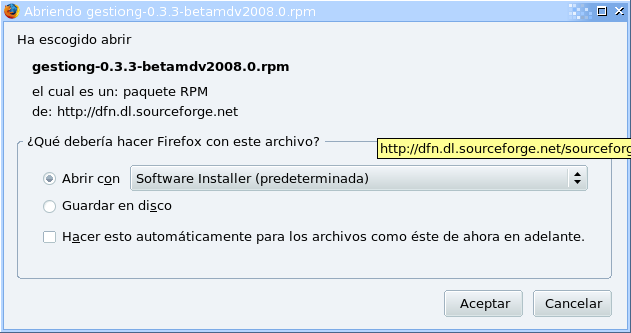
\includegraphics[width=7.964cm,height=4.643cm]{manual-img2.png}
\end{center}
\begin{center}
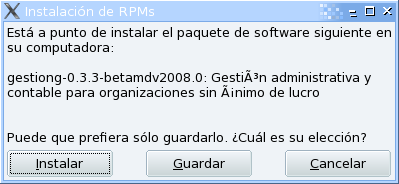
\includegraphics[width=8.345cm,height=3.928cm]{manual-img3.png}
\end{center}
\begin{center}
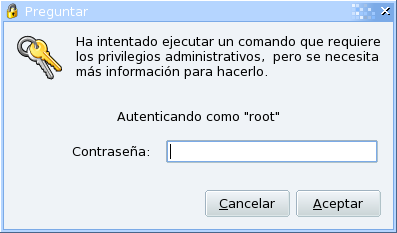
\includegraphics[width=7.758cm,height=4.648cm]{manual-img4.png}
\end{center}
\begin{center}
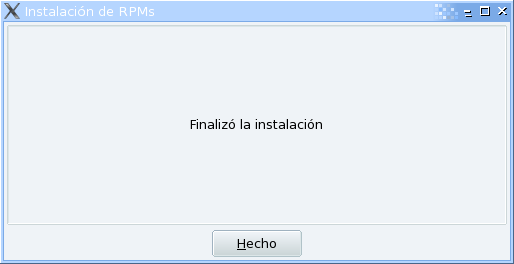
\includegraphics[width=8.56cm,height=4.489cm]{manual-img5.png}
\end{center}

\bigskip


\bigskip


\bigskip


\bigskip


\bigskip


\bigskip


\bigskip


\bigskip



\begin{center}
\begin{minipage}{16.919cm}
{\centering\bfseries\itshape
\label{ref:accesoroot}Acceso a root
\par}

En los sistemas operativos multiusuaria del tipo GNU/Linux hay una
usuaria especial llamada \textbf{\textit{root}} que tiene permiso para
hacerlo todo. Puede instalar y eliminar programas, agregar y quitar
hardware, acceder a cualquier fichero y en general realizar cualquier
tarea administrativa. El resto de usuarias tiene un conjunto de
permisos más reducido, por lo que para ciertas operaciones necesitan
acceder al ordenador como \textbf{\textit{root}}, y por lo tanto deben
conocer su contraseña o bien pedir a la usuaria
\textbf{\textit{root}} que realice esas operaciones.

En la consola las órdenes \textbf{sudo} y \textbf{su} sirven para
ejecutar comandos como si fueras \textbf{root}, preguntando previamente
su contraseña, como verás más adelante.
\end{minipage}
\end{center}
En caso de no instalarse automáticamente, guarda el paquete en tu
carpeta de inicio o personal (o {\textquotesingle}Home
Folder{\textquotesingle}), abre una consola (lee el recuadro !`Abre una
consola! en la página \pageref{ref:abreunaconsola}), y dependiendo de
tu distribución:

{\bfseries\itshape
Mandriva, Fedora y Red Hat:}



\begin{center}
\begin{minipage}{16.48cm}
\textstyleUserEntry{\$ cd}

\textstyleUserEntry{\$ su}

\textstyleUserEntry{password:}\textstyleUserEntry{
\ \ }\textstylekonsolecomment{(escribe la contraseña de root y pulsa
Intro, ATENCION: NO SE VERÁ LO QUE ESCRIBAS)}

\textstyleUserEntry{\# rpm -ihv
}\textstyleUserEntry{gestiong-0.3.3-r0mdv2008.0.rpm}

\textstyleUserEntry{\$ exit}
\end{minipage}
\end{center}

\bigskip


\bigskip


\bigskip

{\bfseries\itshape
Debian, Ubuntu, Kubuntu, GuadaLinex.}



\begin{center}
\begin{minipage}{16.48cm}
\textstyleUserEntry{\$ cd}

\textstyleUserEntry{\$ sudo dpkg -i
}\textstyleUserEntry{gestiong\_0.3.3-r0\_i386.deb}

\textstyleUserEntry{password:}\textstyleUserEntry{
\ \ }\textstylekonsolecomment{(escribe la contraseña de root y pulsa
Intro, ATENCION: NO SE VERÁ LO QUE ESCRIBAS)}
\end{minipage}
\end{center}
Si todo ha funcionado correctamente, lee el apartado Creando un enlace a
GestiONG en el escritorio en la página \pageref{ref:creaenlace}.

\subsection{Construyendo el programa}
\label{ref:construyendoprograma}Si no hay paquetes disponibles para tu
sistema o no están actualizados, puedes construir tú misma el
programa a partir de sus fuentes. Si sabes cómo hacerlo, estas son
las instrucciones:



\begin{center}
\begin{minipage}{16.48cm}
\textstyleUserEntry{\$ cd}

\textstyleUserEntry{\$ mkdir gongsrc}

\textstyleUserEntry{\$ cd gongsrc}

\textstyleUserEntry{\$ wget
}\href{http://dfn.dl.sourceforge.net/sourceforge/gestiong/gestiong-0.3.3-alfa.tar.gz}{\textstyleUserEntry{http://dfn.dl.sourceforge.net/sourceforge/gestiong/gestiong-0.3.3-r0.tar.gz}}

\textstyleUserEntry{\$ tar -zxvf gestiong-0.3.3-r0.tar.gz}

\textstyleUserEntry{\$ cd gestiong-0.3.3}

\textstyleUserEntry{\$ ./configure -{}-prefix=/usr/local}

\textstyleUserEntry{\$ make}

\textstyleUserEntry{\$ sudo make install}

\textstyleUserEntry{\$ gestiong}
\end{minipage}
\end{center}

\bigskip


\bigskip


\bigskip


\bigskip


\bigskip


\bigskip


\bigskip

Dependiendo de tu familiaridad con GNU/Linux puedes entender o no este
proceso, pero aún sin entender nada, siguiendo las instrucciones a
continuación deberías ser capaz de construirlo. Si estás
totalmente perdida, es absolutamente necesario que leas primero el
recuadro \textit{!`Abre una consola!}. 

\begin{center}
\begin{minipage}{16.947cm}
{\centering\bfseries\itshape
\label{ref:abreunaconsola}!`Abre una consola!
\par}

En el mundo de GNU/Linux, todas las operaciones de administración del
ordenador (instalar programas, instalar una impresora, añadir
usuarias, configurar el acceso a Internet, hacer copias de seguridad,
etc.) se pueden realizar tanto con programas gráficos (con botones,
colores y usando el ratón) como tecleando comandos desde una ventana
con fondo negro y letras blancas (o viceversa) conocida como \textit{la
consola}. No es necesario conocer estos comandos para utilizar un
sistema GNU/Linux, pero en algún momento de tu vida alguien te
dirá: {\textquotedblleft}\textit{Abre una
consola}{\textquotedblright} y entrarás de lleno en el mundo del
hacking.

Dependiendo del escritorio que utilices la abrirás de una forma
distinta. Para \textbf{\textit{Gnome}}, pulsa
\textstyleGUIELEMENTREDUCED{Alt+F2 }y escribe \textbf{gnome-terminal} y
pulsa \textstyleGUIELEMENTREDUCED{Intro} (o elige desde el menú
principal: \textstyleGUIELEMENTREDUCED{Aplicaciones$\rightarrow
$Accesorios$\rightarrow $Terminal}).\textstyleGUIELEMENTREDUCED{ }En
KDE, pulsa \textstyleGUIELEMENTREDUCED{Alt+F2} \ (o elige la opción
{\textquotesingle}\textstyleGUIELEMENTREDUCED{Ejecutar
orden}{\textquotesingle} del menú principal), escribe
\textbf{konsole} y pulsa \textstyleGUIELEMENTREDUCED{Intro}. 



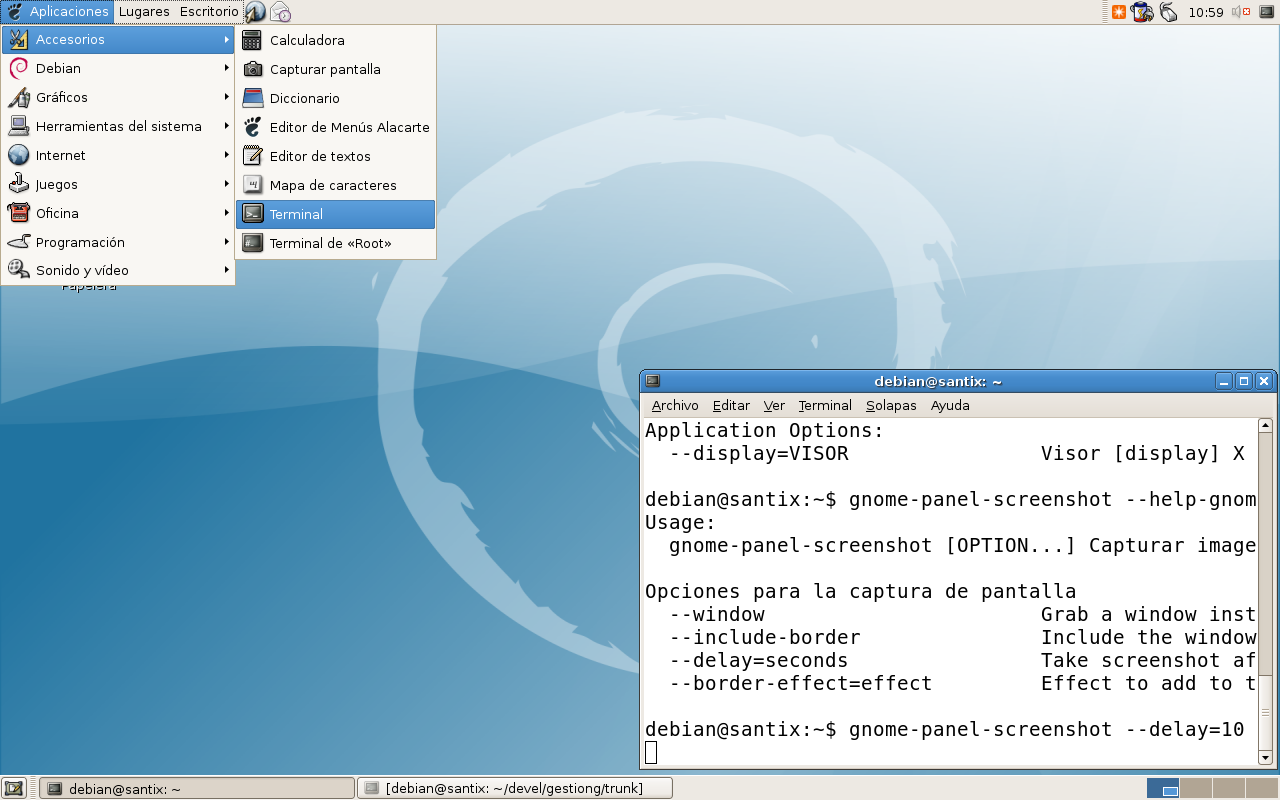
\includegraphics[width=7.915cm,height=4.946cm]{manual-img6.png}
\captionof{figure}[El escritorio de Gnome]{El escritorio de Gnome}
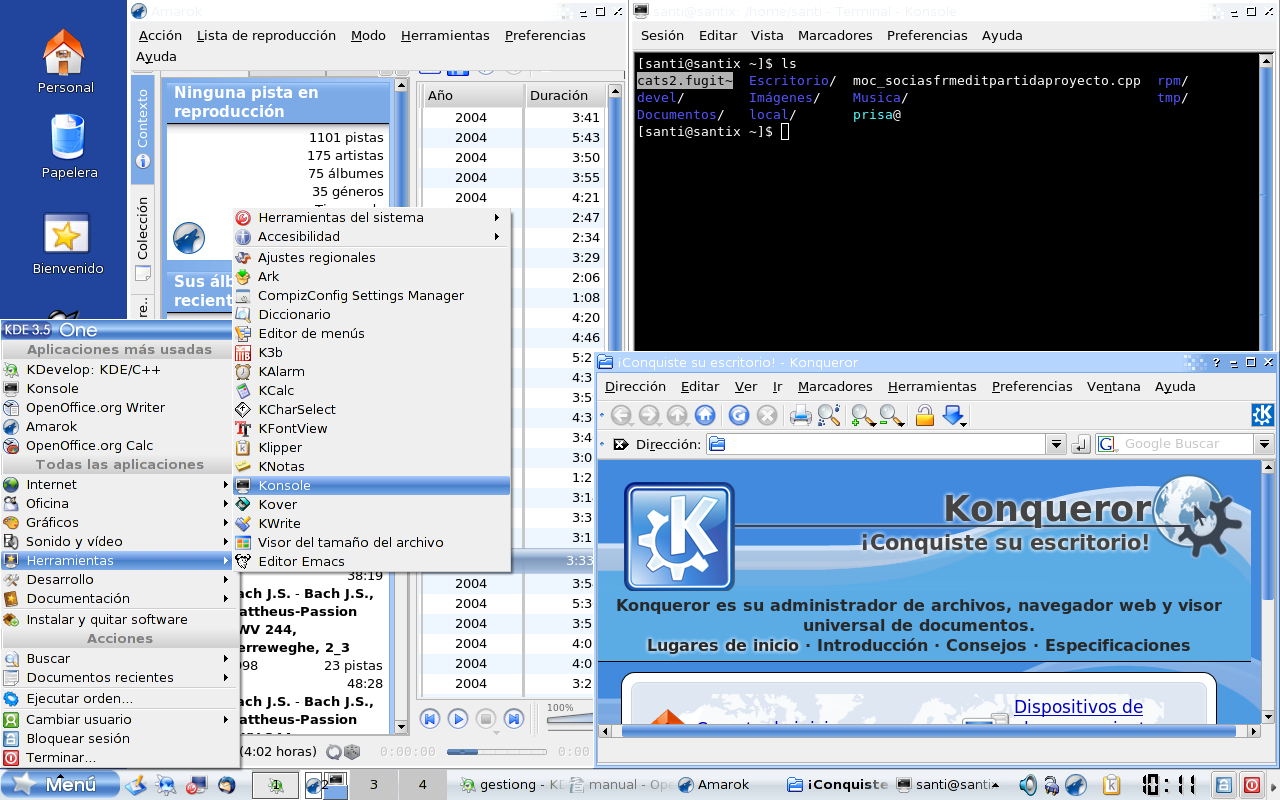
\includegraphics[width=7.953cm,height=4.868cm]{manual-img7.png}
\captionof{figure}[El escritorio de KDE]{El escritorio de KDE}
En la consola estableces una comunicación con el ordenador, a su
manera. Éste presenta una línea acabada con un símbolo de dólar
y un cursor parpadeante donde puedes escribir órdenes o comandos.
Cada vez que escribas una orden \textbf{debes pulsar}
\textstyleGUIELEMENTREDUCED{Intro} para que el ordenador la interprete
y muestre el resultado o un mensaje de error. Escribe la orden
\textbf{ls} (una ele y una ese) y pulsa
\textstyleGUIELEMENTREDUCED{Intro }y observa lo que aparece. Ahora
escribe \textbf{cmderroneo} y observa el mensaje de error. Cuando
quieras cerrar la consola, escribe el comando \textbf{exit}.

Ya estás preparada para realizar cualquier operación desde la
consola. En este manual, los comandos que necesitas ejecutar en una
consola se mostrarán dentro de un cuadro como este:

donde se ha suprimido la parte a la izquierda del \$ ya que en cada
ordenador será diferente. Tienes que escribir lo que hay a la derecha
del símbolo de dólar respetando todos los guiones, espacios,
puntos, etc. Si la orden es complicada, siempre puedes copiar y pegar.
Al final de cada línea, pulsa \textstyleGUIELEMENTREDUCED{Intro}.
\begin{minipage}{16.489cm}
\textstyleUserEntry{\$ cd gongsrc \ \ }\textstylekonsolecomment{(Aquí
a la derecha pueden aparecer algunas aclaraciones)}

\textstyleUserEntry{\$ ls }\ \ \textstylekonsolecomment{(que no tienes
que teclear)}
\end{minipage}\end{minipage}
\end{center}
\clearpage\paragraph{Descargando el programa}
Antes de comenzar, mediante la consola, vas a crear una carpeta dentro
de tu carpeta personal o de inicio (o {\textquotesingle}\textit{Home
Folder}{\textquotesingle}) que se llamará
{\textquotesingle}\textit{gongsrc}{\textquotesingle} donde realizarás
todo el proceso de construcción. \textit{!`Abre una consola!} y
teclea lo siguiente: (recuerda que solamente tienes que teclear lo que
hay a la derecha del símbolo del dólar):



\begin{center}
\begin{minipage}{16.48cm}
\textstyleUserEntry{\$ cd}

\textstyleUserEntry{\$ mkdir gongsrc}

\textstyleUserEntry{\$ cd gongsrc}
\end{minipage}
\end{center}

\bigskip

Ahora tienes que conseguir el fichero comprimido que contiene el
código fuente para la versión que vas a instalar:
\textit{gestiong-0.3.3-r0.tar.gz}. Puedes descargarlo con tu navegador
favorito desde la página:

\ \ \url{http://sourceforge.net/project/showfiles.php?group_id=80104&package_id=81685&release_id=578703}



\bigskip

y guardarlo en la carpeta gongsrc que acabas de crear en tu carpeta
personal.


\bigskip

Aunque es más fácil y rápido descargarlo desde la consola
utilizando el comando wget: 



\begin{center}
\begin{minipage}{16.48cm}
\textstyleUserEntry{\$ wget
http://dfn.dl.sourceforge.net/sourceforge/gestiong/gestiong-0.3.3-r0.tar.gz}
\end{minipage}
\end{center}
Independientemente de cómo consigas el fichero, una vez descargado y
grabado en la carpeta
{\textquotesingle}\textit{gongsrc}{\textquotesingle}, tienes que
descomprimirlo con las siguientes órdenes:

\paragraph[]{}
\begin{center}
\begin{minipage}{16.856cm}
\textstyleUserEntry{\$ tar -zxvf
gestiong-0.3.3-r0.tar.gz}\textstyleUserEntry{\ \ }\textstylekonsolecomment{(Aparecerán
muchas letras muy rápidas...)}

\textstyleUserEntry{\$ cd gestiong-0.3.3}
\end{minipage}
\end{center}
\paragraph{Preparando el entorno para la construcción}
Si no has realizado nunca el proceso de construcción de un programa en
tu ordenador, lo más probable es que necesites instalar una serie de
herramientas de programación, para lo cual necesitarás
\textbf{acceso a Internet} y la contraseña de root (ver
recuadro\textit{ }\textit{Acceso a root}\textit{ }en la página
\pageref{ref:accesoroot}):

Según tu distribución, esto es lo que tienes que hacer (recuerda que
necesitas acceso a Internet):



\begin{center}
\begin{minipage}{16.701cm}
{\itshape
\ \ \textstylekonsolecomment{(Para las distribuciones K/Ubuntu/Debian de
GNU/Linux:)}}

\textstyleUserEntry{\$ sudo aptitude install build-essential
libqt3-mt-dev libboost-dev }

\textstyleUserEntry{password:}\textstyleUserEntry{
\ \ }\textstylekonsolecomment{(escribe la contraseña de root y pulsa
Intro, ATENCION: NO SE VERÁ LO QUE ESCRIBAS)}

\textstyleUserEntry{\$ sudo aptitude install libxml2-dev
libmysqlclient15-dev libdb4.5-dev}


\bigskip

{\itshape
\ \ \textstylekonsolecomment{(Para la distribución Mandriva de
GNU/Linux:)}}

\textstyleUserEntry{\$ su}

\textstyleUserEntry{password:}\textstyleUserEntry{
\ \ }\textstylekonsolecomment{(escribe la contraseña de root y pulsa
Intro, ATENCION: NO SE VERÁ LO QUE ESCRIBAS)}

\textstyleUserEntry{\# urpmi make gcc-c++ libqt3-devel libboost1-devel}

\textstyleUserEntry{\# urpmi libxml2-devel libmysql-devel
libdb4.5-devel}

\textstyleUserEntry{\$ exit}

{\itshape
\textstylekonsolecomment{\ \ (Para las distribucies Fedora y Red Hat de
GNU/Linux:)}}


\bigskip
\end{minipage}
\end{center}

\bigskip


\bigskip

\paragraph{Compilando}
Antes de compilar las fuentes del programa, tienes que decidir si lo vas
a instalar en modo local (para una sola usuaria) o en modo global (para
todas las usuarias de tu ordenador). Normalmente lo querrás instalar
en modo global, reservando el modo local para cuando no tienes acceso a
\textit{root}. (Ver el recuadro {\textquotedblleft}\textit{Acceso a
root}{\textquotedblright}).

Si lo vas a instalar globalmente, ejecuta los siguientes comandos (el
comando \textbf{make }tardará bastante y escribirá un montón de
basurilla; sabrás que ha terminado cuando vuelva a aparecer el prompt
\$):



\begin{center}
\begin{minipage}{16.48cm}
\textstyleUserEntry{\$ ./configure }

\textstyleUserEntry{\$ make}

\textstyleUserEntry{\$ sudo make install}

\textstyleUserEntry{password: \ \ }\textstylekonsolecomment{(escribe la
contraseña de root y pulsa Intro, ATENCION: NO SE VERÁ LO QUE
ESCRIBAS)}
\end{minipage}
\end{center}

\bigskip


\bigskip

Si lo vas a instalar localmente:



\begin{center}
\begin{minipage}{16.48cm}
\textstyleUserEntry{\$ ./configure -{}-prefix=\$HOME/local}

\textstyleUserEntry{\$ make}

\textstyleUserEntry{\$ make install}
\end{minipage}
\end{center}

\bigskip


\bigskip


\bigskip

!`Enhorabuena! Ya tienes GestiONG instalado en tu ordenador. Ahora
puedes ponerlo en marcha, pero recuerda que para poder trabajar con
él, necesitas primero instalar la base de datos.

\paragraph{Ejecutando GestiONG}
Dependiendo del tipo de instalación que hayas elegido para GestiONG,
local o global, el programa estará en un lugar distinto. 

En global, ejecuta simplemente:



\begin{center}
\begin{minipage}{16.48cm}
\textstyleUserEntry{\$ \ gestiong}
\end{minipage}
\end{center}

\bigskip

En local, teclea este comando (teclea también el dólar delante de
HOME):



\begin{center}
\begin{minipage}{16.48cm}
\textstyleUserEntry{\$ \ \$HOME/local/bin/gestiong}
\end{minipage}
\end{center}

\bigskip


\bigskip

\subsection{Creando un enlace a GestiONG en el escritorio}
\label{ref:creaenlace}De nuevo aquí, dependiendo de tu distribución
de GNU/Linux, la operación será algo distinta. Pero se puede
reducir básicamente a dos escritorios, KDE y GNOME (si utilizas otro
entorno, seguro que sabes crear el acceso directo).

Haz click con el botón derecho del ratón en un área vacía del
escritorio y:

a) para KDE, selecciona, {\textquotesingle}\textstyleGUIELEMENT{Crear
Nuevo...}{\textquotesingle}
({\textquotesingle}\textstyleGUIELEMENT{Create
New...}{\textquotesingle}) y luego
{\textquotesingle}\textstyleGUIELEMENT{Enlace a
aplicación...}{\textquotesingle}
({\textquotesingle}\textstyleGUIELEMENT{Link to
application...}{\textquotesingle}). Haz click sobre la pestaña
{\textquotesingle}\textstyleGUIELEMENT{Aplicación}{\textquotesingle}
({\textquotesingle}\textstyleGUIELEMENT{Application}{\textquotesingle}).

b) para Gnome: selecciona {\textquotesingle}\textstyleGUIELEMENT{Crear
un lanzador...}{\textquotesingle}
({\textquotesingle}\textstyleGUIELEMENT{Create
New...}{\textquotesingle}).

En el recuadro
{\textquotesingle}\textstyleGUIELEMENT{Comando}{\textquotesingle}
({\textquotesingle}\textstyleGUIELEMENT{Command}{\textquotesingle})
escribe la localización del programa \textit{gestiong}. Si lo has
instalado desde un paquete preparado para tu sistema o lo has
construido globalmente, escribe simplemente \textit{gestiong}. Si lo
has construido en local, escribe \textit{\$HOME/local/bin/gestiong.}
Pulsa el botón
{\textquotesingle}\textstyleGUIELEMENT{Aceptar}{\textquotesingle}
({\textquotesingle}\textstyleGUIELEMENT{Ok}{\textquotesingle}) y ya
tendrás en tu escritorio el enlace a GestiONG.

\clearpage\subsection{Instalando el servidor de la base de datos}
\label{ref:instalandosqlserver}Dependiendo del número y localización
de los ordenadores de tu organización, quizás sea necesario
instalar la base de datos en uno de ellos. Los escenarios más
frecuentes con los que te puedes encontrar son:

\begin{center}
\begin{minipage}{7.687cm}
{\centering\bfseries\itshape
¿Qué es el servidor de la base de datos?
\par}

Los datos con los que trabajan aún muchas asociaciones suelen estar
contenidos en varias hojas de cálculo: la hoja de socias, la de
gastos, etc. lo cual presenta ciertos inconvenientes, como acceso
incontrolado, duplicidad de datos, imposibilidad de actualizaciones
simultáneas, descentralización, etc.

GestiONG usa un sistema de base de datos independiente llamado MySQL
(www.mysql.com), el cual permite entre otras cosas:

\liststyleLiv
\begin{enumerate}
\item almacenamiento centralizado de los datos,
\item el acceso solo a usuarias identificadas,
\item el acceso desde cualquier ordenador conectado a la red local o a
través de Internet,
\item una capacidad prácticamente ilimitada de almacenamiento.
\end{enumerate}
Con GestiONG se pueden gestionar múltiples asociaciones, cada una con
su correspondiente base de datos que pueden estar localizadas en
diversos lugares.
\end{minipage}
\end{center}
\liststyleLv
\begin{enumerate}
\item \begin{enumerate}
\item Si solamente tenéis un ordenador en vuestra asociación,
tendréis que instalar tanto la base de datos como GestiONG en el
mismo ordenador, que actuará como servidor.
\item Si tenéis varios ordenadores conectados en red, solo será
necesario instalar la base de datos en uno de ellos, que asumirá el
papel de servidor y podréis instalar GestiONG en el resto de
ordenadores conectados a aquél.
\item También podéis tener la base de datos fuera de la oficina, por
ejemplo, cuando se instala en la sede central de la organización o
cuando habéis contratado el servicio de base de datos con una empresa
externa. En ese caso, la central o la empresa proveedora os
facilitará la información necesaria para conectar con el servidor.
\end{enumerate}
\end{enumerate}

\bigskip

Para los escenarios a) y b), necesitarás acceso como \textit{root} al
ordenador donde vas a instalar el servidor (lee el recuadro
{\textquotedblleft}\textit{Acceso a root}{\textquotedblright} en la
página \pageref{ref:accesoroot} si no estás familizarizada con este
concepto). \textit{!`Abre una consola!} en ese ordenador y ejecuta lo
siguiente:



\begin{center}
\begin{minipage}{16.48cm}
{\itshape
\textstylekonsolecomment{\ \ (Para las distribuciones K/Ubuntu/Debian de
GNU/Linux:)}}

\textstyleUserEntry{\$ sudo apt-get install mysql-server}

{\itshape
\textstylekonsolecomment{\ \ (Para la distribución Mandriva de
GNU/Linux:)}}

{\itshape
\textstyleUserEntry{\textup{\$ su}}}

{\itshape
\textstyleUserEntry{\textup{\$ urpmi mysql}}}
\end{minipage}
\end{center}

\bigskip


\bigskip

Ahora, pon una contraseña a la superusuaria del servidor de la base de
datos (sustituye el texto \ \textit{tunuevacontraseña} por la
contraseña que quieres poner):



\begin{center}
\begin{minipage}{16.48cm}
\$ mysqladmin password \textit{tunuevacontraseña}
\end{minipage}
\end{center}

\bigskip


\bigskip

Si has optado por el escenario b), necesitas saber la dirección IP de
este ordenador, conocido como \textit{servidor de la base de datos}.
Ejecuta este comando \ y anota los cuatro números que aparecen tras
\textbf{inet addr:}, algo así \ como 192.168.1.120.



\begin{center}
\begin{minipage}{16.48cm}
\textstyleUserEntry{\$ su}

\textstyleUserEntry{\# ifconfig eth0 {\textbar} grep
{\textquotedblleft}inet addr{\textquotedblright} {\textbar} grep -v
127{\textbackslash}.}

\textstyleUserEntry{\# exit}
\end{minipage}
\end{center}

\bigskip


\bigskip

Recuerda estos datos para cuando tengas que crear la base de datos de
GestiONG más adelante: para los escenarios a) y b) la contraseña
que has puesto a la superusuaria; para el escenario b) además, la
dirección IP del servidor donde has instalado MySQL; para el
escenario c), esta información te la proporcionarán externamente. 

\chapter{Poniendo en marcha \appname}

\label{ref:poniendoenmarcha}\subsection[El asistente de acceso]{El
asistente de acceso}

\begin{center}
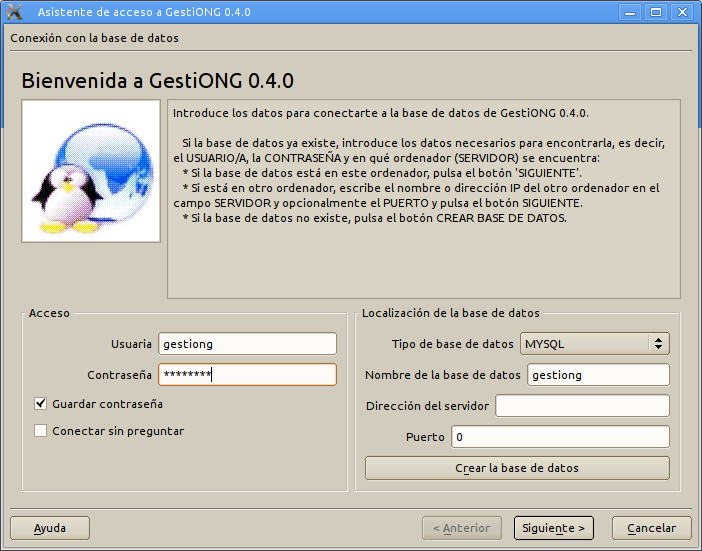
\includegraphics[width=12cm]{bienvenidaagestiong.png}
\captionof{figure}{Asistente de acceso a \appname}
\label{seq:refIllustration3}
\end{center}

Cada vez que ejecutas \appname en tu ordenador, aparece el
{\textquotedblleft}\textbf{\textit{Asistente de acceso a
\appname}}\textbf{{\textquotedblright}} para controlar el acceso a la
base de datos de vuestra asociación. Si la base de datos ya existe, tienes que indicar 
su nombre (\textstyleGUIELEMENT{Nombre de la base de datos}), en qué ordenador
(\textstyleGUIELEMENT{Dirección del servidor} y \textstyleGUIELEMENT{Puerto}) se
encuentra, el nombre de una \textstyleGUIELEMENT{Usuaria} autorizada y
su \textstyleGUIELEMENT{Contraseña} y después pulsar el botón
\textstyleGUIELEMENT{Siguiente (Next)}. 

Sin embargo, la primera vez que ejecutas \appname en tu
asociación, tienes que crear la base de datos. Para ello, necesitas
saber la \textstyleGUIELEMENT{Contraseña de la superusuaria} del
servidor de la base de datos. Los escenarios más frecuentes con los
que te puedes encontrar a la hora de crear la base de datos son, como
has visto en el apartado \textit{Instalando el servidor de la
base de datos}:

\liststyleLv
\begin{enumerate}
\item Si solamente tenéis un ordenador en vuestra asociación,
habrás instalado tanto la base de datos como \appname en el mismo
ordenador, que actuará como servidor:
\end{enumerate}

\textstyleGUIELEMENTREDUCED{NOMBRE DE LA BASE DE DATOS}: gestiong

\textstyleGUIELEMENTREDUCED{DIRECCIÓN DEL SERVIDOR}: (vacío)

\textstyleGUIELEMENTREDUCED{PUERTO}: 0

\textstyleGUIELEMENTREDUCED{NOMBRE DE LA UPERUSUARIA}: root

\textstyleGUIELEMENTREDUCED{CONTRASEÑA DE LA SUPERUSUARIA}: (la que
hayas puesto al servidor MySQL al instalarlo o vacía por defecto)

\liststyleLv
\setcounter{saveenum}{\value{enumi}}
\begin{enumerate}
\setcounter{enumi}{\value{saveenum}}
\item Si tenéis varios ordenadores conectados en red, habrás
instalado la base de datos en uno de ellos, que asumirá el papel de
servidor y podréis instalar \appname en el resto de ordenadores:
\end{enumerate}

\textstyleGUIELEMENTREDUCED{NOMBRE DE LA BASE DE DATOS}: gestiong

\textstyleGUIELEMENTREDUCED{DIRECCIÓN DEL SERVIDOR}: (la dirección
IP del servidor de la base de datos, algo como 192.168.1.120)

\textstyleGUIELEMENTREDUCED{PUERTO}: 0

\textstyleGUIELEMENTREDUCED{NOMBRE DE LA SUPERUSUARIA}: root 

\textstyleGUIELEMENTREDUCED{CONTRASEÑA DE LA SUPERUSUARIA}: (la que
hayas puesto al servidor MySQL al instalarlo o vacía por defecto)

\liststyleLv
\setcounter{saveenum}{\value{enumi}}
\begin{enumerate}
\setcounter{enumi}{\value{saveenum}}
\item También podéis tener la base de datos fuera de la oficina, por
ejemplo, en la sede central de la organización o si habéis
contratado el servicio de base de datos con una empresa externa. En ese
caso, la central o la empresa proveedora os facilitará la
información necesaria para crear la base de datos:
\end{enumerate}

\textstyleGUIELEMENTREDUCED{NOMBRE DE LA BASE DE DATOS}: (proporcionada
por tu proveedora)

\textstyleGUIELEMENTREDUCED{DIRECCIÓN DEL SERVIDOR}: (proporcionado
por tu proveedora, algo como mysql.midominio.org u 84.123.12.34)

\textstyleGUIELEMENTREDUCED{PUERTO}: 0

\textstyleGUIELEMENTREDUCED{NOMBRE DE LA UPERUSUARIA}: (proporcionada
por tu proveedora)

\textstyleGUIELEMENTREDUCED{CONTRASEÑA DE LA SUPERUSUARIA}:
(proporcionada por tu proveedora)

\smallskip

Al mismo tiempo que se crea la base de datos de la asociación, se
creará también una \textstyleGUIELEMENT{Usuaria} con su
correspondiente \textstyleGUIELEMENT{Contraseña} para accesos
posteriores ({\textquotesingle}\textit{gestiong{\textquotesingle}} en
el ejemplo de la \textit{\figurename~\ref{seq:refIllustration3}}). Es
posible añadir más usuarias posteriormente, cada una con un nivel
de acceso adecuado a su rol en la asociación. \ 

\subsection[Creando la base de datos]{Creando la base de datos}
Con todos estos datos a mano, puedes ahora comenzar el proceso de
creación de la base de datos utilizando el
{\textquotedblleft}\textbf{\textit{Asistente de acceso a
\appname}}\textbf{{\textquotedblright}}
(\textit{\figurename~\ref{seq:refIllustration3}}). En importante leer
con atención las instrucciones que aparecen en esta ventana y sobre
todo, la información que aparezca en caso de ocurrir algún error.
En el recuadro \textstyleGUIELEMENT{Acceso a \appname} introduce el
nombre de la \textstyleGUIELEMENT{Usuaria} (y la
\textstyleGUIELEMENT{Contraseña}) con la que usarás habitualmente
el programa, en este ejemplo,
{\textquotesingle}\textit{gestiong}{\textquotesingle}. Completa los
datos con un \textit{1} en el \textstyleGUIELEMENT{N{\textordmasculine}
de asociación} y el \textstyleGUIELEMENT{Ejercicio} actual.

En el recuadro \textstyleGUIELEMENT{Localización de la base de datos},
rellena los datos según el escenario de instalación que hayas
elegido de los tres que has visto más arriba. En el ejemplo de la
\textit{\figurename~\ref{seq:refIllustration3}}, la base de datos se
encontraría en tu propio ordenador. 


\bigskip

Ahora pulsa el botón \textstyleGUIELEMENT{Crear la base de datos},
tras lo cual el asistente mostrará esta nueva ventana
(\textit{\figurename~\ref{seq:refIllustration4}}):

\begin{center}
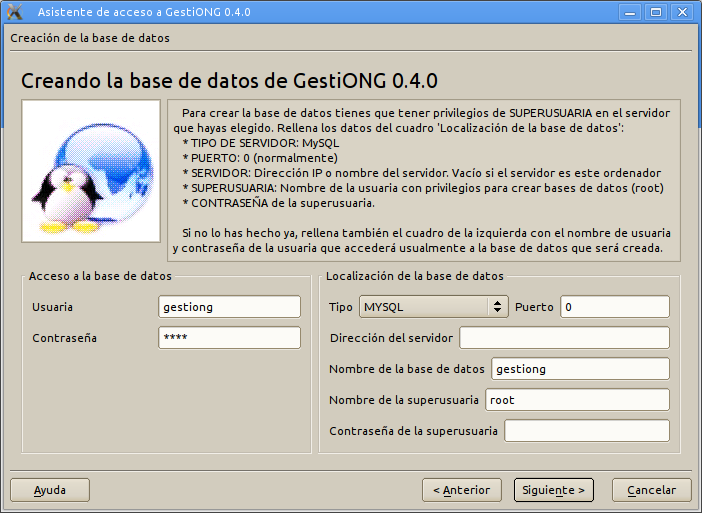
\includegraphics[width=12cm]{creandolabasededatos.png}
\captionof{figure}{Asistente para la creación de la base de datos}
\label{seq:refIllustration4}

\end{center}
En el recuadro \textstyleGUIELEMENT{Localización de la base de datos}
deberás introducir la \textstyleGUIELEMENT{Dirección
del servidor}, el \textstyleGUIELEMENT{Nombre de la superusuaria,} que será casi siempre
{\textquotesingle}\textit{root}{\textquotesingle}, la
\textstyleGUIELEMENT{Contraseña de la superusuaria,} y pulsar el
botón \textstyleGUIELEMENT{Siguiente (Next).} Si todo va bien,
vuestra base de datos se habrá creado correctamente y pasarás a la ventana principal. 


\subsection{La ventana principal}
Ya tienes, por fin, creada la base de datos y la asociación. Ahora
aparece la ventana principal de \appname, el entorno donde trabajarás
con los ficheros y los procesos cotidianos de gestión.

%\chapter{Primeros pasos}

He creado dos empresas, una para la cantina y otra para la tienda y grupo de consumo.



\chapter{Módulo de gestión de la \organizacion}
\label{chap:gestionorganizacion}

Para trabajar con \appname es necesario introducir ciertos parámetros de tu \organizacion. La primera vez que se ejecuta el programa, se crea automáticamente una \organizacion con el código 1 que hay que completar para el correcto funcionamiento:

\medskip

\noindent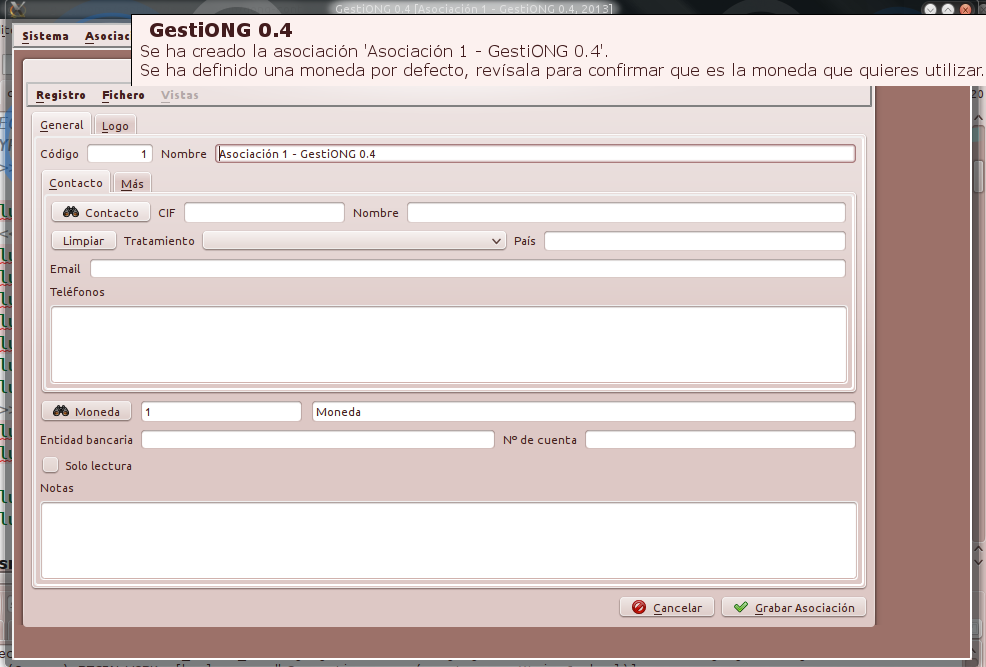
\includegraphics[width=\linewidth]{images/empresainicial.png}

\section{Datos importantes}

\begin{description}
 \item [Nombre] El nombre o razón social de la \organizacion. Puede utilizarse el nombre comercial o un nombre más conocido y más abajo, en el contacto, el nombre jurídico o legal de la \organizacion. Este nombre aparecerá más destacado en el encabezado de las facturas que emitamos. A modo de ejemplo, una persona en el régimen de autónomos introduciría el nombre comercial de su empresa aquí.
 \item [Contacto] Estos son los datos legales de contacto de la \organizacion o de su representante. Aquí introducimos el CIF y el nombre jurídico. A continuación rellenamos todos los datos de la localización de la empresa. Los datos mínimos a  rellenar para poder emitir facturas legales en España son: Nombre, CIF y la dirección completa (Dirección, Localidad y Provincia).
 \item [Moneda] La moneda principal de esta \organizacion. Se pueden definir más monedas y sus tasas de cambio con respecto a la moneda principal.
\end{description}


\section{Datos secundarios}
Cualquiera de los datos a continuación pueden aparecer en los documentos que imprimamos, sin embargo, no son fundamentales para el funcionamiento del programa.
\begin{description}
 \item [email, teléfonos, fax, página web, ...] 
 \item [Entidad bancaria y Nº de cuenta] Representan la entidad y los 20 dígitos de la cuenta bancaria principal de la empresa.
 \item [Logo] Se puede elegir una imagen que aparecerá en los encabezados de los documentos que se impriman.
 \item [Solo lectura] Esta casilla se marca si queremos que no se pueda realizar ninguna operación que cambie el estado de la empresa: compras, ventas, añadir o borrar clientes, etc. Es decir, solo se pueden visualizar datos, pero no se puede modificar nada.
\end{description}


\section{Monedas}

\appname permite trabajar con diferentes monedas, tanto oficiales como complementarias o sociales. Al crear la primera empresa, se crea una moneda por defecto a partir de los valores de la configuración de tu ordenador. Se pueden crear más monedas así como cambiar sus parámetros (por ejemplo, la tasa de cambio con respecto a la moneda principal) desde el menú \menu{Empresa->Moneda}.

\section{Tipos de IVA}

Se puede importar la definición de los tipos de IVA estándar con la opción \menu{Fichero=>Importar} del fichero de Tipos de IVA.

Buscar en la agencia tributaria: Nuevos tipos impositivos en el IVA

\url{http://www.agenciatributaria.es/AEAT.internet/Inicio_es_ES/_Segmentos_/Empresas_y_profesionales/Empresas/IVA/IVA.shtml}

\section{Formas de pago}

La definición de las formas de pago se realiza desde el menú \menu{Sistema->Formas de pago}. Se puede importar una lista predefinida de formas de pago con la opción \menu{Fichero->Importar}.

Formas de pago predefinidas:
\begin{enumerate}
 \item 
  \begin{description}
  \item [Contado] El documento (factura o albarán) se considera pagado por caja con la moneda principal en el mismo momento de ser emitido. No se generará ningún recibo.
  \end{description}
 \item
  \begin{description}
  \item [A reposición] El importe queda pendiente en el documento y se genera un recibo que será pagado en un momento posterior indefinido.
  \end{description}
\end{enumerate}


\chapter{Módulo de gestión de los contactos}

El módulo de gestión de los contactos proporciona una base de datos
personales global y única para toda la organización: personal
contratado, personas socias, voluntarias, acreedoras, etc. o cualquier
otra persona de interés para la organización.

Con este módulo se puede:

\liststyleLvii
\begin{itemize}
\item Añadir y eliminar contactos mecánicamente.
\item Importar y exportar masivamente listas de contactos.
\end{itemize}
Para mantener la base de datos de contactos, ve a
\textstyleGUIELEMENT{Asociación $\rightarrow $ Contactos...}

\section{El fichero de datos personales de los contactos}
Los datos de contacto de las personas físicas o jurídicas de vuestra
organización se almacenan en un fichero aparte del fichero de
miembros de los proyectos. Las ventajas de este diseño son:

\liststyleLviii
\begin{enumerate}
\item Se pueden reutilizar los contactos evitando duplicarlos si tenemos
una persona que es a la vez socia, empleada, acreedora, ...,
\item Toda la información de carácter personal está recogida en un
solo fichero, lo cual es útil para el cumplimento de la LOPD (Ley
Orgánica de Protección de Datos de Carácter Personal), 
\item Si un dato personal cambia, solo hará falta cambiarlo en un
lugar.
\item Se pueden introducir en el sistema contactos que no son socias o
que no tienen ninguna relación administrativa con la organización
\end{enumerate}

\bigskip


% \chapter{Módulo de facturación}

% Facturas: Lo que se va a declarar a Hacienda (lleva IVA, etc.).
% Albaranes: Todo lo demás.
% 
% Tipo de documento: Normal: Todo lo que se va a presentar en Hacienda, al asesor, etc.
%   Serie B: Todo lo demás.
% 
% Número de albarán: Si no tenemos el número, debemos inventarnos uno, la fecha o una brevísima descripción.

El módulo de facturación permite el control del almacén, de las compras y de las ventas de vuestra \organizacion.

\section{Planificando el almacén}

% \marginpar{\small Antes de comenzar asegúrate de que has rellenado todos los datos de tu \organizacion como se detalla en el capítulo \ref{chap:gestionorganizacion}, \titleref{chap:gestionorganizacion} y especialmente los tipos de IVA.}

Los pasos preliminares para facilitar la gestión de la facturación son:

\begin{description}
 \item [Estructurar tu almacén en familias de artículos relacionados.]
Por ejemplo: materias primas, productos de artesanía, alimentación, libros, bebidas, etc. De esta manera, además de tener el almacén mejor organizado, podrás activar o desactivar familias para que aparezcan en el TPV o en Internet; podrás realizar operaciones selectivamente sobre los artículos de una determinada familia, etc. 
 \item [Decidir cómo codificar los artículos.]
Cada artículo debe tener un código único, no demasiado largo pero descriptivo. 

\begin{enumerate}
\item {Si los artículos tienen código de barras, utilízalos directamente.}
\item {Para libros o revistas, utiliza el código ISBN, que suele coincidir con el código de barras.}
\item {Para el resto, utiliza el código o referencia propio de la proveedora. Como es muy probable que se repitan los códigos de diversas proveedoras, antepón a cada código las dos o tres primeras letras del nombre de la proveedora. Esto se puede hacer fácilmente desde la plantilla de carga masiva de artículos (ver más adelante)}.
\item {Para artículos que no tienen ningún tipo de código, puedes crear tú tus propios códigos. \appname permite definir una serie de criterios para cada proveedora para crear los códigos de sus artículos de forma automática.}
\end{enumerate}

\end{description}

\section{Carga masiva de datos de artículos}

Aunque \appname está diseñado para que la introducción de datos sea lo más rápida y sencilla posible, la carga inicial de cientos o miles de artículos es un proceso muy costoso que se puede aligerar utilizando una plantilla de importación de artículos que viene con \appname \footnote{La plantilla se encuentra en \filename{\tiny /usr/share/gonglib/gong-factu/plantillas/import/ARTICULO.xls}}.

Esta plantilla se debe rellenar con datos que se pueden conseguir de diversas formas:

\marginpar{\small Conviene llamar por teléfono a tus proveedoras para insistir en la necesidad y urgencia de recibir el fichero de artículos.}

\begin{enumerate}
 \item {\textbf{Solicita a tus proveedoras un fichero con los datos de sus artículos}. Los datos a pedir son, como mínimo:
 \begin{itemize}
  \item Referencia del producto (Código de barras, ISBN, código interno, etc. )
  \item Nombre 
  \item Coste
  \item Tipo de IVA
  \item Familia o categoría
  \item Fabricante
 \end{itemize}
 }
 \item {Busca en la página web de la proveedora las referencias en un formato de tabla como una hoja de cálculo o una tabla que se pueda copiar o pegar (no vale .PDF).}
 \item {Algunas proveedoras proporcionan hojas de pedido con sus productos.}
 \item {Recopila albaranes o facturas de compra recientes}.
 \item {Rellena a mano la plantilla de artículos}.
\end{enumerate}

Una vez que hayas conseguido estos datos, ve copiando las columnas a la plantilla. Las columnas de la plantilla que hay que rellenar obligatoriamente son:

\begin{description}
 \item [ARTICULO.CODIGO] {El código del artículo. \par 
 \truco{
 Puedes anteponer varias letras del nombre de la proveedora a los códigos de los artículos, puedes hacerlo de la siguiente manera:
 \begin{enumerate}
  \item Crea una nueva columna junto a la de ARTICULO.CODIGO, que será la columna \textbf{B}.
  \item Copia en esa nueva columna los códigos de los artículos
  \item Si quieres anteponer, por ejemplo, el texto \textit{ABC}, crea la fórmula \filename{=``ABC'' \& B2} en la casilla A2.
  \item Arrastra esa fórmula en la columna A hasta completar todos los códigos
\end{enumerate}
 } %truco
 }
 \item [ARTICULO.NOMBRE] {El nombre del artículo.\par
 Algunos artículos de proveedoras distintas pueden tener nombres idénticos. Aunque no es un problema para \appname puesto que al buscar un artículo nos aparecerá una lista donde elegir si hay varios repetidos, sí que es conveniente no tener duplicado el nombre para evitar elegir un artículo de otra proveedora. Se puede utilizar el procedimiento anterior para añadir el nombre de la proveedora o cualquier otro texto al nombre del producto.
 }
 \item [ARTICULO.FAMILIA\_ID] {El código de la familia del artículo.}
 \item [ARTICULO.TIPOIVA\_ID] {El código del tipo de IVA. Normalmente el código coincide con el porcentaje del IVA.}
 \item [ARTICULO.PROVEEDORA\_ID] {El código de la proveedora.}
\end{description}

El resto de columnas no es obligatorio rellenarlas:

\begin{description}
 \item [ARTICULO.CODIGOINTERNO]
 \item [ARTICULO.FABRICANTE] {Fabricante u origen del artículo.}
 \item [ARTICULO.COSTESINIVA, ARTICULO.COSTE] {}
 \item [ARTICULO.MARGENCOMERCIAL] {}
 \item [ARTICULO.PVPSINIVA, ARTICULO.PVP] {}
 \item [ARTICULO.DTOCOMERCIAL] {}
 \item []  {\par No es necesario rellenar todos los precios. Si se rellena el coste o PVP sin IVA, el programa calculará el coste o PVP con IVA. Si se rellena el coste y el margen comercial, se calculará el PVP. Si se rellena el PVP y el descuento comercial, se calculará el coste.}
 \item [ARTICULO.STOCKINICIAL] {Las existencias del artículo en el momento de poner en marcha \appname. Hay que llevar cuidado con no incluir aquí existencias si luego vamos a introducir los albaranes de compra o venta de estos artículos, puesto que se sumaría o restaría otra vez la cantidad en el albarán.}
 \item [ARTICULO.CONTROLAREXISTENCIAS] {Escribe un 1 si quieres que se controlen las existencias de este artículo, o un 0 si no.}
 \item [ARTICULO.STOCKMINIMO, ARTICULO.STOCKMAXIMO] {Las existencias mínimas y máximas deseadas de ese artículo.}
 \item [ARTICULO.NOTAS] {Cualquier comentario adicional sobre el artículo.}
 \item [ARTICULO.PARATPV] {Escribe un 1 si quieres que aparezca en la pantalla del TPV, o un 0 si no.}
\end{description}

% \subsection{Familias de artículos}
% 
% Se accede al fichero de mantenimiento de familias desde el menú \menu{Facturación => Familias}. Los datos a rellenar son:
% 
% \section{Tipos de documentos}
% 
% \appname maneja los cuatro documentos típicos del ciclo de facturación, tanto para compras como para ventas: presupuestos (sólo para ventas), pedidos, albaranes y facturas. 
% 
% 

\section{Informes}

He estudiado el tema del informe de ventas y he "descubierto" lo 
siguiente: 

* El informe va factura por factura viendo los artículos, y sumando el 
precio al que se han vendido (incluyendo el descuento en ese 
artículo). Va sumando el precio sin iva y el precio con iva. 
* Luego muestra el total de esa suma. 

Pero en la factura se añaden otros datos que están fuera de cada 
artículo, que son el recargo de equivalencia y el descuento total que 
se hace en la factura. Estos dos valores no se tienen en cuenta en el 
listado de artículos. Para tenerlos en cuenta, tendría que hacer lo 
siguiente: 

* Para cada artículo que se ha vendido, ver en su factura si había 
recargo de equivalencia y sumárselo (esto es un coñazo pero se puede 
hacer). 
* Para cada artículo que se ha vendido, ver si se ha hecho descuento 
en su factura. Entonces, si hay descuento, aplicárselo a cada artículo 
proporcionalmente (el porcentaje). También es un coñazo, y también se 
puede hacer. 

Pero yo me pregunto si es necesario que salga lo mismo. A ver, en el 
listado que sacas de las facturas de venta, tienes precisamente lo que 
has facturado, que incluye recargos, iva y descuentos. En el informe 
de ventas, tienes datos globales sobre ventas de artículos, sin tener 
en cuenta si luego ha habido descuentos por otros conceptos que ya no 
tienen que ver con el artículo. 

En fin, esto sirve para aclararnos. Si crees que es necesario que en 
ambos listados coincida la cantidad, puedo hacerlo, poniendo una 
casiila que diga [ ] incluir descuentos y recargos de la factura. 




\chapter{Módulo de gestión de proyectos y socias}

\bigskip

El módulo de gestión de proyectos y socias permite:

\liststyleLix
\begin{itemize}
\item Mantener la base social de vuestra organización.
\item Definir diferentes proyectos: talleres, cursos, proyectos de
cooperación, etc.
\item Asignar cuotas a las socias para generar remesas de recibos.
\item Generar ficheros de remesas para el procesamiento automatizado por
parte de bancos y cajas de ahorro.
\item Gestionar los pagos, impagos y devoluciones de los recibos.
\item Definir el formato de las partidas de gastos e ingresos para
presentar a la entidad financiadora.
\item Asignar los diferentes gastos e ingresos a las diferentes
partidas.


\bigskip
\end{itemize}
\section{Proyectos, socias y socios}
\appname considera a las personas socias de vuestra organización como
miembros de un determinado proyecto, en vez de presentar un apartado
específico para su gestión. Esta generalización permite tratar
todos los proyectos de la misma forma: añadir miembros, remesas,
recibos, cuotas, cuadros de financiación y de gastos, etc. \ Dentro
de la categoría de proyectos caben tanto talleres y jornadas a las
que es preciso inscribir miembros, como proyectos de cooperación con
entidades financiadoras, personal expatriado, cooperantes, etc. o
cualquier otro tipo de proyectos. En general, un proyecto es cualquier
acción de vuestra organización que está compuesta por personas,
que pueden tener o no una cuota por participar en ella y que tiene
asociada una partida de gastos e ingresos.

Desde este punto de vista, la base social de vuestra organización es
un proyecto más cuyos miembros son las personas socias.


\bigskip

\subsubsection{El fichero de proyectos}
Para añadir tanto vuestra base social como otro tipo de proyectos ve
al menú \textstyleGUIELEMENT{Asociación $\rightarrow $
Proyectos...} (ver \textit{Añadiendo algunos datos básicos},
página \pageref{ref:aadiendoalgunosdatosbasico}). Además de los
datos identificativos del proyecto, las fechas de alta y/o baja y el
estado, podrás añadir información para la posterior generación
de cuotas. Veamos algunos ejemplos de proyectos:

\paragraph{Base social de la organización}
Debes crear un proyecto para añadir a las personas socias de tu
organización cuyo nombre podría ser precisamente el de tu
organización. Una vez creado, selecciona la pestaña
\textstyleGUIELEMENT{M}\textstyleGUIELEMENT{iembros} y pulsa el botón
\textstyleGUIELEMENT{Añadir }para ir añadiendo socias. También
puedes importar los datos masivamente como se explica en el apartado
\textit{Importando masivamente datos de socias y socios} (página
\pageref{ref:Importandomasivamente}) del capítulo
\textbf{\textit{Poniendo en marcha \appname}}\textbf{\textit{.}} La
\textstyleGUIELEMENT{Fecha de inicio} del proyecto puede ser la de la
creación de vuestra organización, el \textstyleGUIELEMENT{Estado}
activo y la \textstyleGUIELEMENT{Fecha de fin} vacía. Si piensas
emitir recibos para el cobro de las cuotas, introduce el
\textstyleGUIELEMENT{Importe} y la \textstyleGUIELEMENT{Periodicidad de
la cuota} estándar. 

\paragraph{Proyecto de cooperación al desarrollo financiado por el
Ayuntamiento}
En estos proyectos, lo habitual es que la entidad financiadora requiera
una justificación de gastos Asociación $\rightarrow $e ingresos
según un formato establecido por ella estructurado en partidas. Como
cualquier otro proyecto, ve al menú \textstyleGUIELEMENT{Asociación
$\rightarrow $ Proyectos... }\textstyleGUIELEMENT{\textmd{\textup{y
rellena la información correspondiente. Activa la pestaña
}}}\textstyleGUIELEMENT{P}\textstyleGUIELEMENT{artidas}\textstyleGUIELEMENT{\textmd{\textup{
y añade las diferentes partidas de gastos e ingresos siguiendo la
estructura de la entidad financiadora. Lee el apartado
}}}\textstyleGUIELEMENT{\textmd{\textup{\ref{ref:Partidasproyectos}}}}\textstyleGUIELEMENT{\textmd{\textup{Partidas
de gastos e ingresos de
proyectos}}}\textstyleGUIELEMENT{\textmd{\textup{ para más
información.}}}

\paragraph[Jornadas]{\bfseries\itshape Jornadas}
Crea un proyecto con la \textstyleGUIELEMENT{Fecha de inicio} y
\textstyleGUIELEMENT{Fecha de fin} de las jornadas y pon el
\textstyleGUIELEMENT{Estado} activo. Si, como es habitual, el nombre de
las jornadas es largo, utiliza un nombre abreviado en el campo
\textstyleGUIELEMENT{Descripción} y el nombre completo en el campo
\textstyleGUIELEMENT{Descripción larga}. Si las jornadas son de pago,
introduce el \textstyleGUIELEMENT{Importe} y la
\textstyleGUIELEMENT{Periodicidad de la
cuota}\textstyleGUIELEMENT{\textmd{\textup{, que será
}}}\textstyleUserEntry{Puntual}\textstyleGUIELEMENT{\textmd{\textup{
caso de ser una sola cuota.}}}

\textstyleGUIELEMENT{\textmd{\textup{Ahora, activa la pestaña
}}}\textstyleGUIELEMENT{Miembros}\textstyleGUIELEMENT{\textmd{\textup{
y añade a las personas inscritas en las jornadas.}}}

\paragraph{Cursos}
Como en el caso de las jornadas, crea un proyecto con el nombre del
curso y añade los miembros al mismo. Si, por ejemplo, se trata de un
curso de pago de nueve meses en el que se paga mensualmente un importe
de \textstyleUserEntry{10{\texteuro}}, introduce en
\textstyleGUIELEMENT{Importe}, 10{\texteuro}, en
\textstyleGUIELEMENT{Periodicidad de la cuota},
\textstyleUserEntry{MENSUAL}\textstyleGUIELEMENT{ }y en
\textstyleGUIELEMENT{Número de cuotas}, \textstyleUserEntry{9.}

\subsubsection{El fichero de miembros de proyectos}
En este fichero se define el tipo de afiliación de cada socia a cada
proyecto, es decir, el tipo de socia, el estado: activo o inactivo, las
fechas de alta y de baja, la cuota y la forma de pago y cuenta
bancaria, en su caso, para el cobro de las cuotas.

Mediante el tipo de socia y la forma de pago se puede gestionar todas
las variedades de pagos de recibos que se pueden presentar en la
asociación. Lee el apartado \ref{ref:Remesasyrecibos} Remesas y
recibos para más información.

\section{Remesas y recibos}
\label{ref:Remesasyrecibos}\appname permite un control fiel de los
cobros de las cuotas de cualquier proyecto, ya sean las cuotas
periódicas de nuestra organización o las cuotas puntuales de una
jornada o las cuotas mensuales de un curso anual. \ Toda esta variedad
de cuotas se define mediante información general del proyecto e
información particular de cada miembro.

\subsubsection{Definición de las cuotas de los proyectos}
Al crear un proyecto, se define el importe y periodicidad de las cuotas
estándar. Veamos algunos ejemplos:

\paragraph{Base social de la organización}
Si tu organización solicita a sus miembros el pago de una cuota anual
de 60{\texteuro}, definiríamos el valor de
\textstyleGUIELEMENT{Importe} a \textstyleUserEntry{60} y el de
\textstyleGUIELEMENT{Periodicidad de la cuota} a
\textstyleUserEntry{anual}. El \textstyleGUIELEMENT{Número de cuotas}
quedaría a cero puesto que no hemos definido una fecha de fin para el
proyecto. 

Los casos particulares a la hora de pagar la cuota, como cuotas
reducidas o formas de pago aplazadas o en distintas entregas, se
definirían posteriormente en la ficha de cada miembro del proyecto.

\paragraph[Curso]{Curso}
Imagina un curso de nueve meses impartido por vuestra organización por
un importe total de 900{\texteuro}. Si quieres generar los recibos del
curso cada mes, \ define el valor de \textstyleGUIELEMENT{Importe} a
\textstyleUserEntry{90}, el de \textstyleGUIELEMENT{Periodicidad de la
cuota} a\textstyleUserEntry{ mensual} y el
\textstyleGUIELEMENT{Número de cuotas }a \textstyleUserEntry{9}. Si
los quieres generar cada trimestre, haz \textstyleGUIELEMENT{Importe} =
\textstyleUserEntry{270}, \textstyleGUIELEMENT{Periodicidad de la
cuota} =\textstyleUserEntry{ trimestral} y
\textstyleGUIELEMENT{Número de cuotas =} \textstyleUserEntry{3}. Si
los quieres anuales, haz \textstyleGUIELEMENT{Importe} =
\textstyleUserEntry{900}, \textstyleGUIELEMENT{Periodicidad de la
cuota} =\textstyleUserEntry{ anual} y \textstyleGUIELEMENT{Número de
cuotas =} 1.

\paragraph{Taller de fin de semana}
En este caso, quieres cobrar una sola cuota de inscripción al taller
de 10{\texteuro}. Haz \textstyleGUIELEMENT{Importe} =
1\textstyleUserEntry{0}, \textstyleGUIELEMENT{Periodicidad de la cuota}
=\textstyleUserEntry{ puntual }y \textstyleGUIELEMENT{Número de
cuotas =} 1.


\bigskip

\subsubsection{Definición de la forma de pago de cada socia}
En el apartado anterior has definido el importe, número y periodicidad
de las cuotas estándar de cada proyecto. Pero cada miembro puede
decidir pagar las cuotas de forma distinta, además de poder acogerse
a reducciones del importe de la cuota por diferentes motivos. Estos
casos particulares se definen utilizando los ficheros de Tipos de socia
y de Formas de pago.

\paragraph{El fichero de tipos de socia}
Para cada miembro es obligatorio definir un tipo de socia que permite,
aparte de clasificarlos, definir el porcentaje sobre la cuota total del
proyecto que deben pagar. Por ejemplo, si la gente desempleada paga
solo el 50\% de la cuota, crea un nuevo tipo de socia desde el menú
\textstyleGUIELEMENT{Asociación $\rightarrow $ Tipos de socia... }al
que puedes llamar \textstyleUserEntry{Personas desempleadas} y en el
campo \textstyleGUIELEMENT{\% cuota} introduce un
\textstyleUserEntry{50}. Ten en cuenta que el campo
\textstyleGUIELEMENT{\% cuota} se refiere al porcentaje que se paga, no
a la reducción. Así, si un tipo de socia tiene una reducción del
30\% del importe de la cuota, debes introducir un 70\%.

\paragraph{El fichero de formas de pago}
Hasta ahora has definido el importe de las cuotas y su periodicidad
según está definido en tu organización. Pero es probable que las
socias decidan pagar las cuotas con una periodicidad menor a la que has
definido. Para ello puedes crear distintas formas de pago desde el
menú \ \textstyleGUIELEMENT{Contabilidad$\rightarrow $ Formas de
pago... }donde puedes definir el número de plazos y el intervalo de
días entre ellos.

Es obligatorio definir una forma de pago para cada miembro. La forma
más habitual será la del que paga las cuotas en un solo plazo
cuando se le presentan. Para ello, define una forma de pago con el
valor \textstyleUserEntry{1} en el campo \textstyleGUIELEMENT{Número
de plazos}.

Para permitir a las socias pagar una cuota anual de forma semestral,
basta con definir la periodicidad de la cuota en el proyecto a anual y
una forma de pago para la socia que incluya dos plazos.

\subsubsection{Emisión de remesas de recibos}
Una vez definidos todos los datos anteriores: Importe, número y
periodicidad de las cuotas en el proyecto, porcentaje de cuota a
aplicar a la socia y forma de pago, puedes generar una remesa de
recibos. 

Por diseño, todos los recibos en \appname deben pertenecer a una
remesa, aunque ésta contenga un solo recibo. Por lo tanto, crea una
nueva remesa desde la pestaña
\textstyleGUIELEMENT{R}\textstyleGUIELEMENT{emesas} que aparece cuando
entras a modificar un proyecto. También puedes hacerlo desde
\textstyleGUIELEMENT{Asociación }\textstyleGUIELEMENT{$\rightarrow
$}\textstyleGUIELEMENT{ Proyectos ...}.

Introduce los datos para identificar la remesa: el proyecto a la que
pertenece, el número, la descripción y las fechas de emisión y de
cargo de los recibos. Si esta remesa va a ser enviada a una caja de
ahorros o banco para su cobro, introduce el código de la cuenta
bancaria donde queréis que sean ingresados los importes de los
recibos.

Una vez guardada la remesa, puedes añadir recibos de dos maneras:
manual y automáticamente. Aunque vas a utilizar casi siempre la forma
automática, comenzaremos explicando la forma manual para que te
familiarices con los recibos y porque en alguna ocasión necesitarás
añadir un sólo recibo.

\paragraph{Añadiendo recibos manualmente}
Entra en \textstyleGUIELEMENT{Asociación
}\textstyleGUIELEMENT{$\rightarrow $}\textstyleGUIELEMENT{ Proyectos
... }y modifica el proyecto y pulsa en la pestaña
\textstyleGUIELEMENT{R}\textstyleGUIELEMENT{emesas} y modifica la
remesa a la que quieres añadir los recibos. Pulsa el botón
\textstyleGUIELEMENT{Añadir recibo}.

\begin{center}
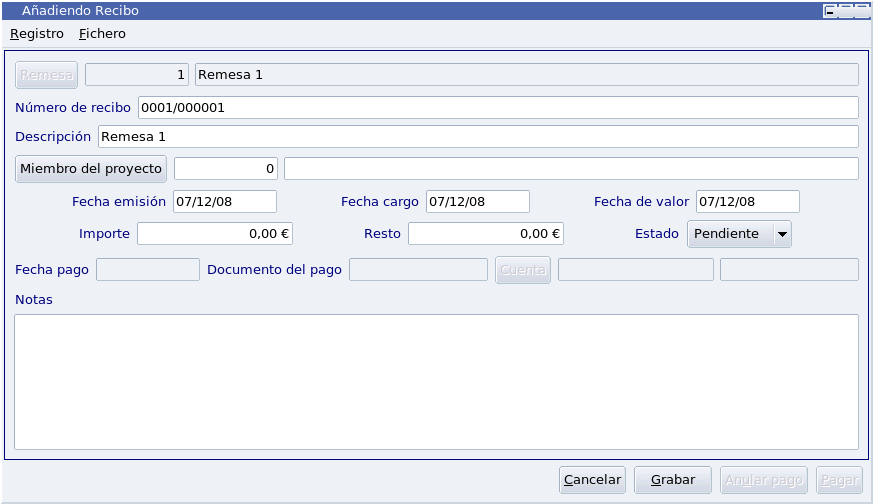
\includegraphics[width=11.956cm,height=7.419cm]{manual-img20.png}
\captionof{figure}[Dando de alta un recibo]{Dando de alta un recibo}

\end{center}
En principio, el número y la descripción del recibo, así como las
fechas de emisión, cargo y valor, \ aparecen automáticamente,
aunque puedes cambiarlas.

Elige el miembro e introduce el importe y resto del recibo. 

La fecha de valor es útil para saber a qué periodo de emisión
pertenece el recibo para evitar emitir recibos duplicados.

\paragraph{Generando remesas automáticamente}
\appname permite generar remesas con los recibos de todos o una parte de
los miembros un proyecto mediante la opción del menú
\textstyleGUIELEMENT{Asociación }\textstyleGUIELEMENT{$\rightarrow
$}\textstyleGUIELEMENT{ Generar recibos ...}

\begin{center}
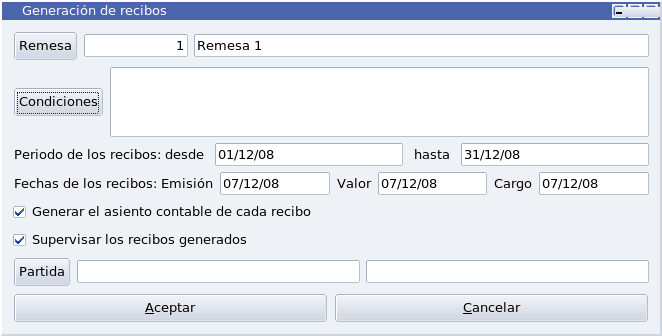
\includegraphics[width=10.261cm,height=5.041cm]{manual-img21.png}
\captionof{figure}[Generando recibos automáticamente]{Generando
recibos automáticamente}

\end{center}
Elige la remesa que contendrá los recibos y, si quieres seleccionar
una parte de los miembros del proyecto, hazlo pulsando el botón
\textstyleGUIELEMENT{Condiciones}. \ Si no, se generarán recibos para
todos los miembros. Introduce el período para el cual se generarán
los recibos y las fechas de emisión, valor y cargo de los mismos. 

Si quieres generar los asientos contables correspondientes a los
recibos, marca la casilla \textstyleGUIELEMENT{Generar
}\textstyleGUIELEMENT{el asiento contable de cada recibo}. Si además,
quieres que los asientos se asignen a una determinada partida de
ingresos del proyecto, elígela. Por último, si quieres revisar los
recibos generados uno por uno antes de que se graben, marca la casilla
\textstyleGUIELEMENT{Revisar los recibos generados}. 

\subsubsection{Envío de remesas a la entidad financiera}
Entra en \textstyleGUIELEMENT{Asociación
}\textstyleGUIELEMENT{$\rightarrow $}\textstyleGUIELEMENT{ Proyectos
... }y modifica el proyecto y pulsa en la pestaña
\textstyleGUIELEMENT{R}\textstyleGUIELEMENT{emesas} y selecciona la
remesa del proyecto que quieres enviar a la entidad financiera para el
tratamiento informatizado de los cobros.

Asegúrate de que has introducido el código de cuenta de abono de tu
caja de ahorros o banco. Revisa también que has introducido el
código de la cuenta bancaria de cada miembro al que quieres cargarle
el recibo. Pulsa el botón \textstyleGUIELEMENT{Generar CB19}. 

Aparecerá una ventana para que introduzcas el nombre y el lugar donde
se va a guardar el \ fichero que has de enviar a la entidad bancaria.
Una vez finalizado el proceso, un mensaje te indicará cuántos
recibos se han generado y cuántos no por diversos motivos: miembro no
activo, númeo de cuenta vacío, etc.

\subsubsection{Gestión de los pagos de los recibos}
Desde el fichero de recibos, ya sea directamente desde
\textstyleGUIELEMENT{Asociación }\textstyleGUIELEMENT{$\rightarrow
$}\textstyleGUIELEMENT{ Recibos ... }o desde\textstyleGUIELEMENT{
Asociación }\textstyleGUIELEMENT{$\rightarrow $}\textstyleGUIELEMENT{
Proyectos }\textstyleGUIELEMENT{$\rightarrow $}\textstyleGUIELEMENT{
Remesas }\textstyleGUIELEMENT{$\rightarrow $}\textstyleGUIELEMENT{
Recibos, }se pueden realizar o anular los pagos. Para realizar el pago
de un recibo pendiente, selecciónalo y pulsa el botón Pagar. A
continuación, introduce la fecha, el importe, el documento y la
cuenta del pago. En estas circunstancias, pueden darse tres casos:

\liststyleLx
\begin{enumerate}
\item El importe introducido coincide con el resto del recibo. El recibo
cambia del estado pendiente al estado pagado y se genera el
correspondiente asiento en contabilidad.
\item El importe introducido es menor que el resto del recibo. El recibo
original queda pagado por la cantidad introducida y se genera un nuevo
recibo con el nuevo resto. Se genera automáticamente el asiento del
pago.
\item El importe introducido es mayor que el resto del recibo. El recibo
original se paga y mientras el importe introducido sea mayor, se eligen
recibos de la misma persona (aunque pueden ser de otros proyectos y/o
remesas) para ir descontando su importe. Al final, se genera un asiento
que recoge todos los pagos conjuntos.
\end{enumerate}

\bigskip

\subsubsection{Impresión del recibí}
Sobre cualquier recibo pagado se puede pulsar CTRL+P para obtener un
informe equivalente a un recibí. El informe se llama recibi.rtk y se
puede personalizar.


\bigskip


\bigskip


\bigskip


\bigskip


\bigskip

\clearpage
\bigskip

\section{Partidas de gastos e ingresos de proyectos}
\label{ref:Partidasproyectos}\label{ref:Partidasproyetos}Para los
proyectos en los que es necesario presentar una justificación de
gastos e ingresos a la entidad financiadora, se pueden definir las
partidas en la pestaña
\textstyleGUIELEMENT{P}\textstyleGUIELEMENT{artidas} del fichero de
proyectos. Para el resto de proyectos, es suficiente con la
contabilidad, aunque también se pueden crear partidas.

Ve al menú \textstyleGUIELEMENT{Asociación
}\textstyleGUIELEMENT{$\rightarrow $}\textstyleGUIELEMENT{ Proyectos
...} y crea o modifica un proyecto. Verás que hay cuatro solapas,
pulsa sobre la última
(\textstyleGUIELEMENT{P}\textstyleGUIELEMENT{artidas}) y verás la
plantilla vacía. Pulsa el botón \textstyleGUIELEMENT{Añadir
partida} y rellena los datos.

Los códigos y las descripciones son totalmente libres aunque no pueden
estar repetidos dentro de un mismo proyecto. Las partidas se pueden
organizar jerárquicamente utilizando el campo
\textstyleGUIELEMENT{Código de la partida madre}, de modo que los
importes que se adjudiquen a esta partida se sumen también a su
partida madre. El \textstyleGUIELEMENT{Tipo }puede ser G para gastos, I
para ingresos y T para el total (Ingresos -- Gastos). El
\textstyleGUIELEMENT{Presupuesto} es útil para compararlo con el
\textstyleGUIELEMENT{Importe} final. Graba la partida y continúa
rellenando la plantilla completamente.

\begin{center}
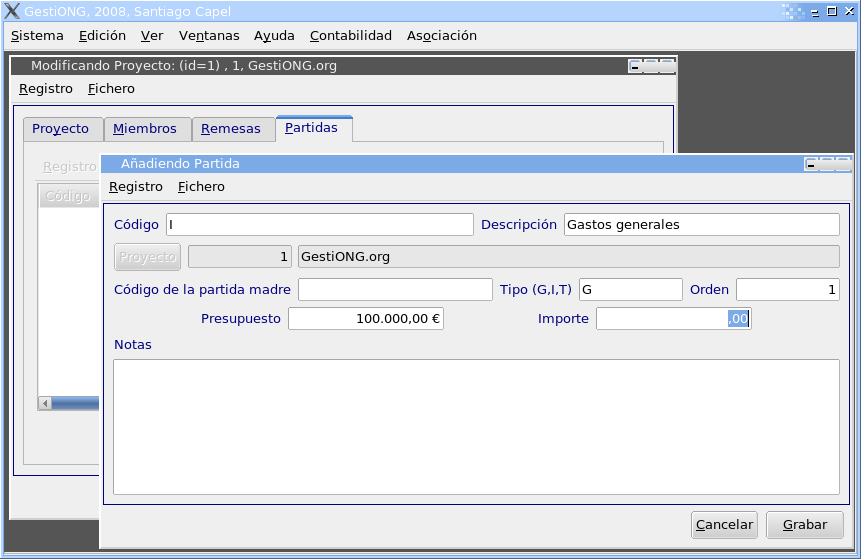
\includegraphics[width=9.738cm,height=6.452cm]{manual-img22.png}
\captionof{figure}[Dando de alta una partida]{Dando de alta una partida}

\end{center}
Se pueden actualizar estas partidas de forma manual para introducir los
gastos e ingresos de cada proyecto y luego realizar un informe para
presentarlo a nuestra financiadora. Sin embargo, lo más fácil es
utilizar el módulo de contabilidad para introducir los movimientos
económicos y asociarlos a partidas de nuestro proyecto, como se
explica en el apartado Asignando apuntes a partidas del capítulo V,
Módulo de contabilidad.

\chapter{Módulo socias}

\subsection{Añadiendo algunos datos básicos}
\label{ref:aadiendoalgunosdatosbasico}El elemento fundamental de
\appname es el proyecto. Un proyecto contiene miembros, tiene una
duración determinada y permite un control económico de gastos e
ingresos. De hecho, todos los socios y socias de tu organización
deberán estar incluidos en un proyecto. Vas a crear este primer
proyecto.

Selecciona el menú \textstyleGUIELEMENT{Asociación $\rightarrow $
Proyectos}, y pulsa el botón \textstyleGUIELEMENT{Añadir}
(\textstyleGUIELEMENT{o Ctrl+A}) en la ventana que aparece. El
\textstyleGUIELEMENT{Código} debería ser el
{\textquotesingle}\textit{1{\textquotesingle}}, tal y como aparece en
la \figurename~\ref{seq:refIllustration6}, la descripción podría
ser {\textquotesingle}\textit{Socios y socias de nuestra
asociación}{\textquotesingle}, la \textstyleGUIELEMENT{Fecha de alta}
la que corresponda y el \textstyleGUIELEMENT{Estado}
{\textquotesingle}\textit{Activo{\textquotesingle}}. Una vez
introducidos todos los datos, pulsa el botón
\textstyleGUIELEMENT{Grabar}.

\begin{center}
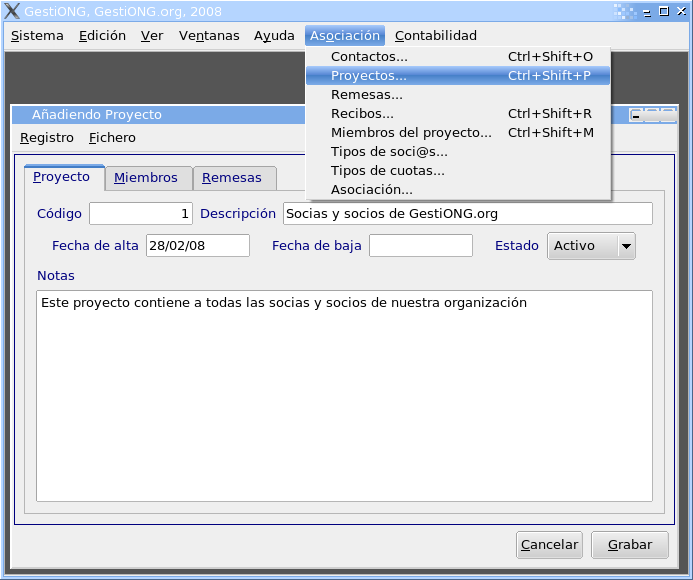
\includegraphics[width=9.618cm,height=6.354cm]{manual-img11.png}
\captionof{figure}[Añadiendo el proyecto principal]{Añadiendo el
proyecto principal}
\label{seq:refIllustration6}

\end{center}
Ahora selecciona el menú \textstyleGUIELEMENT{Asociación
$\rightarrow $ Tipos de
}\href{mailto:soci@s}{\textstyleGUIELEMENT{soci@s}} y añade un tipo
de socia (pulsa \textstyleGUIELEMENT{Ctrl+A}) con
\textstyleGUIELEMENT{Código}
{\textquotesingle}\textit{1}{\textquotesingle} y
\textstyleGUIELEMENT{Descripción}
{\textquotesingle}\textit{Normal}{\textquotesingle}. Selecciona
\textstyleGUIELEMENT{Asociación $\rightarrow $ Tipos de cuotas} y
añade un tipo de cuota con \textstyleGUIELEMENT{Código
{\textquotesingle}}\textit{1}{\textquotesingle} y
\textstyleGUIELEMENT{Descripción} {\textquotesingle}\textit{Cuota
anual}{\textquotesingle} o {\textquotesingle}\textit{Cuota
semestral}{\textquotesingle} o cualquier otro nombre que describa las
cuotas de vuestra asociación, así como el
\textstyleGUIELEMENT{Importe} de las mismas. Si tenéis diferentes
cuotas, da de alta todas ellas. Por último, selecciona
\textstyleGUIELEMENT{Contabilidad $\rightarrow $ Formas de pago} y
añade tantas formas de pago como utilicéis.

Si tienes dificultades para realizar estas operaciones, o quieres dejar
de ser esclava del ratón, lee el recuadro
\textit{{\textquotesingle}Trucos para \ ir más
rápidas{\textquotesingle}}.



\begin{center}
\begin{minipage}{16.794cm}
{\centering\bfseries\itshape
Trucos para ir más rápidas
\par}

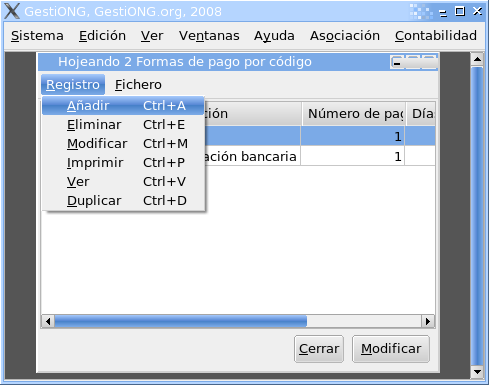
\includegraphics[width=6.332cm,height=5.186cm]{manual-img12.png}
\captionof{figure}[Hojeando formas de pago]{Hojeando formas de pago}
Utilizar el ratón para seleccionar menús, hacer click sobre botones,
ir al siguiente campo, etc. es intuitivo pero lento. La mayoría de
las operaciones tienen uno o varios equivalentes con el teclado. Por
ejemplo, los menús y los botones tienen generalmente una letra
subrayada: se pueden activar pulsando a la vez la tecla \textbf{Alt} y
esa letra subrayada. Por ejemplo, los botones Cerrar (Alt+C) y
Modificar (Alt+M) y los menús de la ventana principal: Sistema
(Alt+S), Ventanas (Alt+N), Asociación (Alt+O), etc.

Cuando un menú se despliega, algunas de sus opciones muestran a la
derecha del nombre una combinación de la tecla \textbf{Ctrl} y una
letra. Pulsar esa combinación de teclas elige esta opción del
menú aunque no esté visible. Por eso, cuando anteriormente pulsabas
\textbf{Ctrl+A} para añadir un registro, en realidad estabas
eligiendo el menú \textstyleGUIELEMENTREDUCED{Registro $\rightarrow $
Añadir}.

Por lo tanto, para añadir una nueva forma de pago utilizando solo el
teclado, pulsa \textbf{Alt+C} (Contabilidad), luego dad al cursor hacia
abajo varias veces hasta llegar a \textbf{Formas de pago...} y entonces
pulsa \textbf{Intro,} tras lo cual aparece la ventana de formas de pago
donde podrás pulsar \textbf{Ctrl+A} o bien \textbf{Alt+R} (Registro)
y luego \textbf{Intro}.
\end{minipage}
\end{center}


\begin{center}
\begin{minipage}{16.794cm}
{\centering\bfseries\itshape
Trucos para ir más rápidas (continuación)
\par}

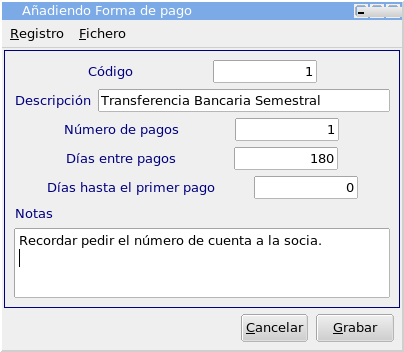
\includegraphics[width=5.877cm,height=5.225cm]{manual-img13.png}
\captionof{figure}[Añadiendo forma de pago]{Añadiendo forma de pago}
Una vez en el formulario para dar de alta la forma de pago, hay unos
recuadros para introducir la información sobre la nueva forma de
pago. Estos recuadros se llaman \textit{campos}. El cursor (indicador
parpadeante de la posición en la que estás tecleando) está ahora
en el campo \textstyleGUIELEMENTREDUCED{Notas}, que puede contener un
texto ilimitado, dividido quizás en párrafos.

Para avanzar al siguiente campo, puedes pulsar la tecla \textbf{Tab}
(tabulador, que se encuentra a la izquierda de la letra \textbf{Q}) o
bien la tecla \textbf{Intro} o bien la tecla \textbf{cursor abajo.}
Para volver al campo anterior, puedes pulsar la tecla \textbf{cursor
arriba} o bien \textbf{Mayús+Tab}. Ten en cuenta que no podrás
salir del campo \textstyleGUIELEMENTREDUCED{Notas}\textit{ }pulsando
\textbf{Intro} porque eso añade una nueva línea: tienes que salir
con \textbf{cursor abajo}, \textbf{Tab} ó
\textbf{Mayús}+\textbf{Tab.}

Una vez introducidos todos los datos necesarios del formulario, puedes
pulsar \textbf{Alt+G }( ó \textbf{F12} )\textbf{ }para
\textstyleGUIELEMENTREDUCED{Grabar} o bien \textbf{Alt+C} ( o
\textbf{Escape} ) para \textstyleGUIELEMENTREDUCED{Cancelar} los datos.
En general, la tecla \textbf{F12} graba o acepta los datos en cualquier
formulario y la tecla \textbf{Escape} los cancela.
\end{minipage}
\end{center}
\subsection{Añadiendo la información del contacto de vuestra
asociación}
Selecciona el menú \textstyleGUIELEMENT{Asociación$\rightarrow
$Contactos...} y pulsa \textstyleGUIELEMENT{Ctrl+A} o el botón
\textstyleGUIELEMENT{Añadir} para introducir un nuevo contacto.
Rellena los datos de vuestra asociación y pulsa
\textstyleGUIELEMENT{Grabar} ó \textstyleGUIELEMENT{F12}. Lee el
recuadro a la derecha para entender por qué los contactos están en
un fichero aparte.

\begin{center}
\begin{minipage}{8.1cm}
{\centering\bfseries\itshape
\label{ref:elficherodecontactos}El fichero de contactos
\par}

La información de carácter personal (nombre, dirección,
teléfonos, email, etc. ) de las personas físicas o jurídicas con
las que trabaja \appname se recogen en un fichero llamado
{\textquotesingle}Contactos{\textquotesingle}. Este fichero se
relaciona, pues, con cualquier otro fichero que tenga datos personales.
Las ventajas de este diseño son varias: se pueden reutilizar los
contactos y se evita duplicarlos si tenemos una persona que es a la vez
una socia y una acreedora; toda la información de carácter personal
está recogida en un solo fichero, lo cual es útil para el
cumplimento de la LOPD; y si un dato personal cambia, solo hará falta
cambiarlo en un lugar.
\end{minipage}
\end{center}
Selecciona ahora el menú \textstyleGUIELEMENT{Asociación
$\rightarrow $ Asociación...} y pulsa el botón
\textstyleGUIELEMENT{Contactos}. Aparece el formulario
{\textquotedblleft}\textbf{\textit{Eligiendo contactos por
CIF{\textquotedblright}}}. Selecciona el contacto que acabas de dar de
alta y pulsa \textstyleGUIELEMENT{Intro.} El \textstyleGUIELEMENT{CIF}
y el \textstyleGUIELEMENT{Nombre} del contacto aparecen en el
formulario de datos de la asociación. Graba.

\subsection{Añadiendo las personas socias }
Una vez grabados todos los datos anteriores, ya puedes comenzar a
añadir miembros a vuestro proyecto, es decir, las socias y socios de
vuestra asociación. Ve a
\textstyleGUIELEMENT{As}\textstyleGUIELEMENT{o}\textstyleGUIELEMENT{ciación$\rightarrow
$Proyectos...}, selecciona el primer proyecto y pulsa el botón
\textstyleGUIELEMENT{M}\textstyleGUIELEMENT{odificar} (o
\textstyleGUIELEMENT{Ctrl+M}). Ahora haz click sobre la pestaña
\textstyleGUIELEMENT{M}\textstyleGUIELEMENT{iembros} (o pulsa
\textstyleGUIELEMENT{Alt+M})\textbf{,} que contiene la lista de
miembros vacía. Pulsa \textstyleGUIELEMENT{Ctrl+A} y aparecerá el
formulario para añadir un nuevo miembro al proyecto.

Fíjate en los títulos de los formularios o ventanas: el que está
activo siempre tiene el fondo azul, en este caso
{\textquotesingle}\textbf{Añadiendo Miembro del
proyecto}{\textquotesingle}. El título ofrece siempre información
valiosa sobre el contenido de la ventana y lo que se está realizando,
por ejemplo, el formulario que está por detrás tiene por título
{\textquotesingle}\textbf{Modificando Proyecto: (id=1), 1, Socias y
socios ...}{\textquotesingle} y está con fondo negro porque su
ventana no está activa en este momento. 

Ahora vas a profundizar un poco más en el proceso de introducción de
datos en \appname tomando como ejemplo el formulario para añadir un
nuevo miembro al proyecto.

El primer campo, \textstyleGUIELEMENT{Proyecto}, está desactivado
porque no se puede cambiar y de ahí su fondo gris. El siguiente
campo, \textstyleGUIELEMENT{N{\textordmasculine} de soci@}, contiene ya
un valor sugerido: el siguiente número de socia disponible. El
siguiente es el \textstyleGUIELEMENT{Contacto}, donde además de poder
introducir un NIF/CIF y/o un nombre, se puede pulsar el botón
\textstyleGUIELEMENT{Contacto} con el ratón ( o
\textstyleGUIELEMENT{F3} ) para buscar el contacto.

\begin{center}
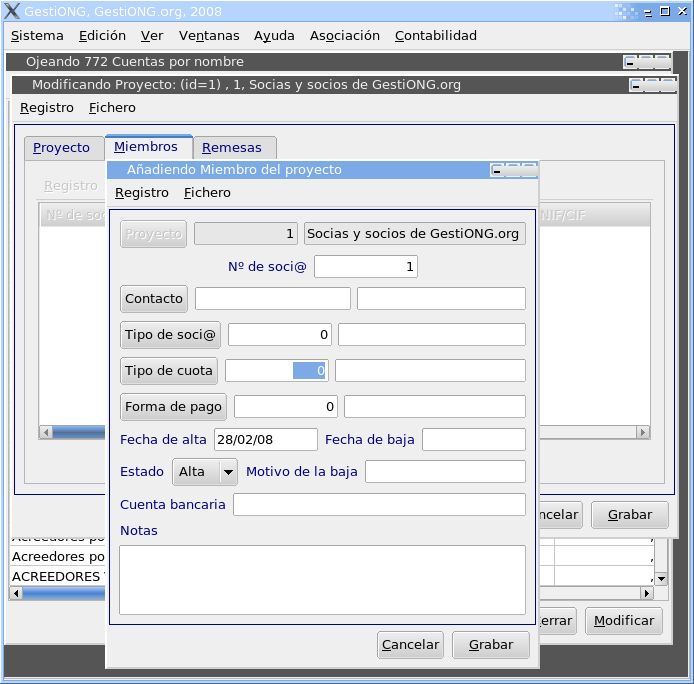
\includegraphics[width=8.772cm,height=8.823cm]{manual-img14.png}
\captionof{figure}[Añadiendo miembro del proyecto]{Añadiendo miembro
del proyecto}

\end{center}
Haz click en el botón \textstyleGUIELEMENT{Contacto} y aparecerá la
ventana del fichero de contactos. Si el que buscas ya estuviera dado de
alta, selecciónalo y pulsa el botón \textstyleGUIELEMENT{Elegir,}
si no, pulsa \textstyleGUIELEMENT{Ctrl+A} para añadir los datos del
contacto correspondiente a la socia o socio número 1. Cuando hayas
rellenado todos los campos, grábalo (botón
\textstyleGUIELEMENT{Grabar}) y elígelo (botón
\textstyleGUIELEMENT{Elegir}). Volverás al formulario de partida con
la información sobre el contacto rellena.

Ahora le toca el turno al \textstyleGUIELEMENT{Tipo de soci@}. Haz click
sobre el botón \textstyleGUIELEMENT{Tipo de soci@} y elige el tipo
apropiado pulsando el botón \textstyleGUIELEMENT{Elegir }o haciendo
\textstyleGUIELEMENT{doble-click} sobre él. Haz lo propio con el
\textstyleGUIELEMENT{Tipo de cuota}. Date cuenta de que cuando estás
eligiendo un contacto, un tipo de soci@ o cualquier otro registro,
puedes igualmente dar de alta nuevos registros pulsando
\textstyleGUIELEMENT{Ctrl+}A o modificarlos pulsando
\textstyleGUIELEMENT{Ctrl+M}.

Pero no siempre es necesario pulsar el botón para elegir un dato. Por
ejemplo, para elegir la forma de pago, puedes teclear un 1 en el
recuadro a la derecha del botón \textstyleGUIELEMENT{Forma de pago},
que es el código, y al pulsar \textstyleGUIELEMENT{Intro},
aparecerá a su derecha la descripción. Igualmente, si escribes la
descripción, aparecerá a la izquierda el código. Puedes incluso
escribir una descripción incompleta, y si existe una forma de pago
que contenga esa descripción incompleta, \appname la encontrará y
la mostrará. Si hubiese más de una forma de pago coincidente,
tendrías la opción de elegir de entre ellas la que andas buscando.
Imagina lo útil que es esto para buscar un contacto del que, por
ejemplo, solo te acuerdas de un apellido.

Vuelve de nuevo al formulario {\textquotedblleft}\textbf{Añadiendo
miembro del proyecto}{\textquotedblright} y rellena los restantes
campos: \textstyleGUIELEMENT{Fecha de alta},
\textstyleGUIELEMENT{Estado}, \textstyleGUIELEMENT{Fecha de baja y}
\textstyleGUIELEMENT{Motivo de la baja} (en su caso),
\textstyleGUIELEMENT{Cuenta bancaria }para el pago de las cuotas, etc.
Graba. Aparece otra vez el mismo formulario en blanco para añadir
otro proyecto. Pulsa la tecla \textstyleGUIELEMENT{Escape} o el botón
\textstyleGUIELEMENT{C}\textstyleGUIELEMENT{ancelar}.

Este es el procedimiento manual para añadir socias a los proyectos,
pero ahora vas a ver cómo puedes importar (introducir
automáticamente) los datos de vuestra hoja de cálculo de socias.

\subsection{Importando masivamente datos de socias y socios}
\label{ref:Importandomasivamente}Si ya tienes los datos de vuestras
socias y socios en una hoja de cálculo (si los tienes en algún otro
tipo de base de datos siempre podrás exportarlos a una hoja de
cálculo o similar) \appname te permite importarlos siempre y cuando
los transformes como se detalla a continuación.

Normalmente, vuestra hoja de cálculo contendrá en una sola hoja
información muy variada sobre las socias, como sus datos de contacto,
número de socia, cuenta bancaria, importe de su cuota, etc. Todos
estos datos se almacenan en ficheros diferentes en \appname, por lo que
habrá que acomodar un poco la hoja de cálculo antes de realizar la
importación. 

\textbf{IMPORTANTE}: \textbf{Realiza una copia de seguridad de tu hoja
original puesto que vas a modificarla sustancialmente.}

Supongamos que vuestra hoja es algo similar a esto:

El primer paso consiste en eliminar las filas iniciales que no contengan
datos de socias, y dejar una primera línea con el encabezado de las
columnas renombradas de forma que \appname sepa qué datos contienen.
Los nombres de las columnas deben coincidir con los nombres internos de
los campos. Para saber cuáles son estos nombres, id a
\textstyleGUIELEMENT{Sistema$\rightarrow $Configuración$\rightarrow
$Diccionario de datos} y aparecerá toda la información necesaria.
Por ejemplo, la columna que contiene el código postal de los
contactos se debe de llamar \textstyleUserEntry{\textit{CONTACTO.CP}}.

\begin{center}
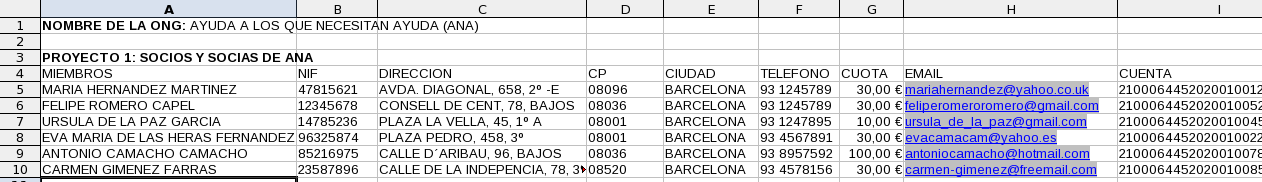
\includegraphics[width=16.999cm,height=2.501cm]{manual-img15.png}
\captionof{figure}[Hoja de socias original]{Hoja de socias original}

\end{center}


\begin{center}
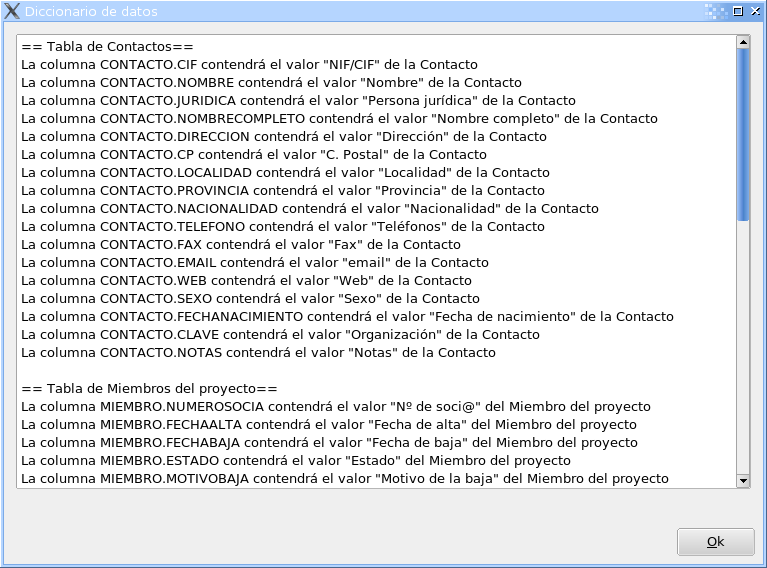
\includegraphics[width=14.328cm,height=10.829cm]{manual-img16.png}
\captionof{figure}[Diccionario de datos]{Diccionario de datos}

\end{center}
Modifica el texto de la primeras fila de cada columna de tu hoja con el
nombre del campo de \appname. Por ejemplo, para el número de socia,
escribe \textstyleUserEntry{MIEMBRO.NUMEROSOCIA}, para el CIF o NIF,
escribe \textstyleUserEntry{CONTACTO.CIF} y así sucesivamente. El
orden de las columnas no importa. 

{\itshape
Atencion: El nombre del socio o socia en \appname se almacena en un solo
campo, por lo tanto, si como en este ejemplo, lo tienes separado en
nombre y apellidos, debes unir ambas columnas.}

Con todos estos cambios realizados, tu hoja tendrá ahora este aspecto:


\bigskip



\begin{center}
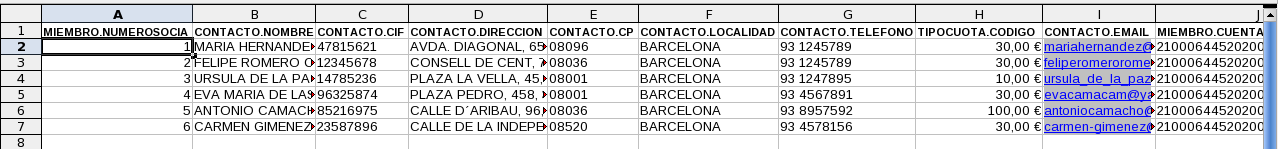
\includegraphics[width=16.999cm,height=2.021cm]{manual-img17.png}
\captionof{figure}[Hoja de socias con los títulos adaptados]{Hoja de
socias con los títulos adaptados}

\end{center}
Lo único que falta es corregir la información sobre los tipos de
cuotas, tipos de socias y formas de pago para que se asocien
correctamente a cada miembro. La columna \textbf{Cuota} de tu hoja
contenía el valor de la cuota en euros, pero debe contener el
código que le has dado en el fichero de tipos de cuota en \appname y
su título debe ser \textstyleUserEntry{TIPOCUOTA.CODIGO}. Búscalo y
corrige su valor para cada socia. Siguiendo este ejemplo,
necesitarías añadir dos nuevas columnas, una que se llamaría
\textstyleUserEntry{TIPOSOCIA.CODIGO} y cuyos valores serían los
códigos con los que habéis dado de alta los tipos de soci@ en
\appname; y otra que se llamaría
\textstyleUserEntry{FORMAPAGO.CODIGO} y contendría los códigos de
las formas de pago. Añade todas las formas de pago, tipos de socia y
cuotas que no estén ya en \appname. Puedes añadir más columnas a
vuestra hoja si posees más información. Por ejemplo, la cuenta
bancaria será la columna \textstyleUserEntry{MIEMBRO.CUENTABANCARIA},
y cualquier otro dato puedes añadirlo en una columna llamada
\textstyleUserEntry{MIEMBRO.NOTAS}.



\begin{center}
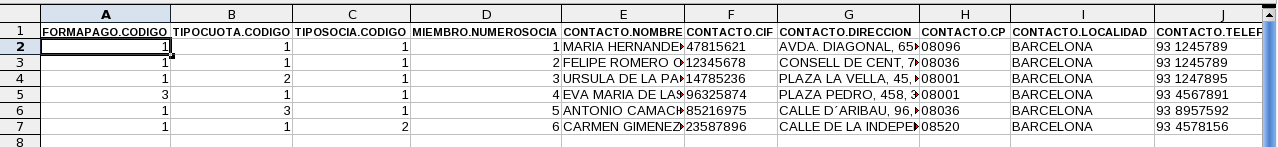
\includegraphics[width=16.999cm,height=1.995cm]{manual-img18.png}
\captionof{figure}[Hoja adaptada totalmente para la importación]{Hoja
adaptada totalmente para la importación}

\end{center}
Una vez adaptada y revisada tienes que guardar la hoja en algún sitio
donde la encuentres posteriormente, con un formato especial: CSV. Desde
\textbf{Openoffice}, ve a \textstyleGUIELEMENT{Archivo$\rightarrow
$Guardar como...}\textbf{, }dale un nombre,\textbf{ }elige el
\textstyleGUIELEMENT{Filtro: Texto CSV} y pulsa
\textstyleGUIELEMENT{Aceptar}. En la ventana que aparece
posteriormente, elige estos valores:



\begin{center}
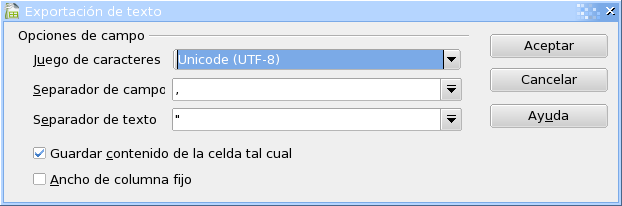
\includegraphics[width=12.748cm,height=4.309cm]{manual-img19.png}
\captionof{figure}[Opciones de exportación a CSV de
OpenOffice]{Opciones de exportación a CSV de OpenOffice}

\end{center}
y pulsa \textstyleGUIELEMENT{Aceptar}.

Ahora, de nuevo desde \appname, realiza primero la importación de los
contactos y luego la de las socias. Ve a
\textstyleGUIELEMENT{Asociación$\rightarrow $Contactos...}, elige la
opción \textstyleGUIELEMENT{Fichero$\rightarrow $Importar} y abre el
fichero CSV que acabas de guardar. \ Antes de comenzar con la
importación, se comprobará que los nombres de las columnas son
correctas y se avisará si has cometido algún error. Si todas las
columnas son correctas, irán apareciendo los contactos uno por uno de
forma que puedas corregir cualquier dato que esté incorrecto o
incompleto. Ve grabando uno por uno los contactos. Cuando hayas
finalizado, ve a \textstyleGUIELEMENT{Asociación$\rightarrow
$Proyectos...}, modifica el proyecto número \textit{1}, ve a la
pestaña de miembros (\textstyleGUIELEMENT{Alt+M}) y luego, bajo esa
pestaña, elige \textstyleGUIELEMENT{Fichero$\rightarrow $Importar...}
Abre el mismo fichero CSV y comenzará la importación de las socias.



\begin{center}
\begin{minipage}{15.189cm}
{\centering\bfseries\itshape
Resumen del proceso de importación de la hoja de socias
\par}

\liststyleLvi
\begin{enumerate}
\item \ Hoja: Poner títulos apropiados (nombre de los campos del
diccionario de datos) a las columnas \ (consultar los nombres en
\appname:\textstyleGUIELEMENTREDUCED{ Sistema$\rightarrow
$Configuración$\rightarrow $Diccionario de datos}).
\item \ \appname: Añadir los tipos de cuota, formas de pago y tipos de
socia que aparezcan en vuestra hoja y que no estén ya dados de alta.
\item \ Hoja: Asegurarse de que existen las columnas
\textstyleUserEntry{TIPOCUOTA.CODIGO, FORMAPAGO.CODIGO y
TIPOSOCIA.CODIGO}. Modificar sus valores para que coincidan con los
códigos en \appname.
\item \ Hoja: Añadir cualquier otro dato relevante sobre las socias,
como la cuenta bancaria, las observaciones, la nacionalidad, los
teléfonos, etc., con su título correspondiente.
\item \ Hoja: Exportarla a un fichero de texto con formato CSV.
\item \ \appname: Importar el fichero CSV desde el fichero de Contactos.
\item \ \appname: Importar el fichero CSV desde la pestaña de
\textstyleGUIELEMENTREDUCED{Miembros del proyecto} del fichero de
proyectos.
\end{enumerate}
\end{minipage}
\end{center}

\chapter{Personalización}
\section{Idioma de la aplicación}
\appname está preparado para mostrar sus mensajes en el idioma que
elija la usuaria. Los idiomas disponibles hasta ahora son: español,
catalán, gallego y euskera, aunque no todos están completos.

El idioma viene predeterminado normalmente en la configuración del
escritorio que utilizas. Si quieres cambiarlo:

a) Si usas KDE, ve a \textstyleGUIELEMENT{Menú K
}\textstyleGUIELEMENT{$\rightarrow $}\textstyleGUIELEMENT{ Centro de
control }\textstyleGUIELEMENT{$\rightarrow $}\textstyleGUIELEMENT{
Regional y accesibilidad }\textstyleGUIELEMENT{$\rightarrow
$}\textstyleGUIELEMENT{ País/Región e idioma}.

\section{Ficheros de configuración globales y locales}
\section{Diccionario de datos: nombres de ficheros y campos }
\appname posee un diccionario de datos con información sobre los
distintos elementos de la base de datos, por ejemplo, los títulos de
las tablas, los tipos y descripciones de los campos, su tamaño, su
estilo, su valor por defecto, etc.

Algunos de los elementos del diccionario de datos se pueden personalizar
modificando unos ficheros de texto con extensión .ddd (Diccionario De
Datos) que se leen al iniciar la aplicación y que se encuentran en el
subdirectorio \textstylenombreprograma{database} del directorio de
configuración general o local. Al modificar esta información, los
cambios se verán reflejados en los menús, formularios e informes de
la aplicación.

Suele haber un fichero por cada módulo de \appname. Así, para el
módulo de socias, el fichero se llama socias.ddd, para el de
contabilidad, conta.ddd y así sucesivamente. Además, se pueden
crear ficheros .ddd para cada idioma que se desee. Basta con anteponer
el código del lenguaje entre guiones bajos al nombre del fichero: por
ejemplo, \_es\_socias.ddd, \_ca\_conta.ddd, etc.

El contenido de esos ficheros es como sigue:



\begin{center}
\begin{minipage}{16.249cm}
\textstyleUserEntry{ASOCIACION.DESC\_SINGULAR=Asociación}

\textstyleUserEntry{ASOCIACION.DESC\_PLURAL=Asociaciones}

\textstyleUserEntry{ASOCIACION.FEMENINA=true}


\bigskip

\textstyleUserEntry{ASOCIACION.CODIGO.CAPTION=Código}

\textstyleUserEntry{ASOCIACION.CODIGO.DESCRIPTION=Código}

\textstyleUserEntry{ASOCIACION.CODIGO.STYLE=CODE}

\textstyleUserEntry{ASOCIACION.CODIGO.WIDTH=0}

\textstyleUserEntry{ASOCIACION.CODIGO.DEFAULTVALUE=}

\textstyleUserEntry{ASOCIACION.NOMBRE.CAPTION=Nombre abreviado
asociación}
\end{minipage}
\end{center}

\bigskip


\bigskip


\bigskip

Las primeras tres líneas definen la tabla de asociaciones, que en la
base de datos se llama
{\textquotedblleft}ASOCIACION{\textquotedblright}. El nombre en
singular de la tabla que aparecerá en \appname será
{\textquotedblleft}Asociación{\textquotedblright}, en plural
{\textquotedblleft}Asociaciones{\textquotedblright} y se declara que el
nombre es femenino. Se podría cambiar
{\textquotedblleft}Asociación{\textquotedblright} por
{\textquotedblleft}Organización{\textquotedblright} y el cambio se
vería reflejado en los menús, formularios e informes.

Las siguientes líneas definen los campos de la tabla de asociaciones.
El campo CODIGO llevará por título
{\textquotedblleft}Código{\textquotedblright}, su descripción
será también {\textquotedblleft}Código{\textquotedblright}, su
estilo {\textquotedblleft}Code{\textquotedblright} y la longitud y el
valor por defecto se dejan sin tocar. A continuación se define el
campo NOMBRE, y así sucesivamente. Un valor muy útil del
diccionario de datos es \textstyleUserEntry{DEFAULTVALUE}, que es el
valor que tomará un campo al ser creado, evitando de este modo tener
que introducirlo cada vez que se da de alta un registro. Por ejemplo,
si ponemos \textstyleUserEntry{CONTACTO.PAIS.DEFAULTVALUE=España},
cada vez que demos de alta un contacto, su país será España.

Inicialmente, \appname instala en el directorio de configuración
global los diccionarios de datos por defecto para diversos lenguajes.
Estos ficheros solo puede modificarlos la superusuaria, por lo que para
cambiarlos, tienes que crear una copia en tu directorio de
configuración local.


\end{document}
